\documentclass[10pt, a4paper]{article}
\usepackage[UTF8]{ctex} % 中文支持
\usepackage{graphicx} % 插入图片
\usepackage{geometry} % 页面设置
\usepackage{amsmath} % 数学公式
\usepackage{booktabs} % 表格美化
\usepackage{float} % 图片表格浮动控制
\usepackage{titlesec} % 标题格式设置
\usepackage{abstract} % 摘要格式
\usepackage{enumitem} % 列表控制
\usepackage{multirow} % 表格多行合并
\usepackage{hyperref} % 超链接

% 页眉：使用 fancyhdr 显示比赛 logo 居中并画一条长下划线，且页脚显示页码
\usepackage{fancyhdr}
\pagestyle{fancy}
\fancyhf{} % 清除默认的页眉页脚
% 居中放置 logo（文件位于 picture/比赛logo.png），根据需要调整 height
\fancyhead[C]{\raisebox{0.1cm}{
\includegraphics[height=1.2cm]{picture/比赛logo.png}}}
% 画一条较粗的头部横线（跨页边距宽度）
\renewcommand{\headrulewidth}{0.6pt}
% 页脚居中显示页码
\fancyfoot[C]{\thepage}
% 增加页眉和正文之间的间距
\addtolength{\headsep}{1.5cm}

% 页面设置
\geometry{left=2.5cm, right=2.5cm, top=3.5cm, bottom=3cm, headheight=0cm}

% 标题格式设置
\titleformat{\section}{\large\bfseries}{\thesection}{1em}{}
\titleformat{\subsection}{\normalsize\bfseries}{\thesubsection}{1em}{}
\titleformat{\subsubsection}{\normalsize\bfseries}{\thesubsubsection}{1em}{}

% 编号格式设置：section保持默认，其他改为1.1、1.2...1.1.1、1.1.2
\renewcommand{\thesection}{
\ifcase\value{section}
\or 第一部分
\or 第二部分
\or 第三部分
\or 第四部分
\or 第五部分
\else 第\arabic{section}部分
\fi
}
\renewcommand{\thesubsection}{\arabic{section}.\arabic{subsection}}
\renewcommand{\thesubsubsection}{\arabic{section}.\arabic{subsection}.\arabic{subsubsection}}

% 摘要格式设置：标题及正文左对齐
\renewcommand{\abstractname}{\large\textbf{摘要}}
\setlength{\absleftindent}{0pt}
\setlength{\absrightindent}{0pt}
\makeatletter
\renewenvironment{abstract}{
    \if@twocolumn
        \section*{\abstractname}
    \else
        \vspace{0.5\baselineskip}\noindent\textbf{\abstractname}\quad\large
    \fi
}{\par}
\makeatother

% 列表格式设置
\setlist[itemize]{topsep=0pt, partopsep=0pt, itemsep=0pt, parsep=0pt}

\begin{document}

% 让首页也使用 fancy 页眉
\thispagestyle{fancy}

% 标题部分
\begin{center}
  \LARGE\textbf{AAA无证电台}

  \vspace{0.5cm}
  \normalsize（不要出现任何涉及学校名称等内容）
\end{center}

% 摘要
\begin{abstract}
    本作品实现了一个基于GOWIN TANG MEGA 138K/60K 与 AD9361 射频前端的端到端无线通信原型系统。系统支持数字基带生成、LVDS 接口的高精度时序对齐、8PSK 基带调制与相应的解调链路、FM广播的接收，并集成了上位机用于寄存器配置与参数可视化。作品能够实现短距离无线通信，设计兼顾了资源占用与性能，适用于教学与科研原型验证、小规模点对点数据/语音传输等应用场景。通过创新的解调方式与流水线优化，实现了低延迟的基带处理与高正确率的网口数据传输。上位机界面友好，支持多种功能模块，提升了系统的易用性与调试效率。
\end{abstract}
\section{作品概述}

\subsection{功能与特性}
本作品实现了可配置的 8PSK 数字基带调制/解调；基带插值/抽取与升余弦成形滤波，解调环路最高可以锁住频偏100KHz-300KHz的信号；LVDS DDR 时序打包与 IODELAY 精细校准；使用以太网传输数据包，实现多设备通信；基于 Python/Qt 的上位机用于寄存器读写、延时与增益调参及运行状态监控；支持FM解调播放等功能，并且能够在低信噪比的情况下正确解调信号。设计兼顾了可移植性与资源占用，兼容 TANG MEGA 138K/60K 两种 FPGA。

\subsection{应用领域}
适用于教学与科研原型验证、小规模点对点数据/语音传输、无线链路算法验证与射频前端校准试验环境。

\subsection{主要技术特点}
采用 AD9361 的 LVDS 数据接口与 GOWIN FPGA 结合实现数字基带处理，利用 ROM 查表实现低延迟的相位映射以节省 DSP 资源；基于多级 CIC + FIR 或可选升余弦滤波满足带外抑制要求；载波相位/频率采用 Costas 环路，符号时钟采用常见的时钟恢复算法，环路参数可在上位机实时调节以适配不同 SNR/频偏条件；上板时序通过 IODELAY 与寄存器配合校准，保证 LVDS 数据/时钟/帧对齐。

\subsection{主要性能指标}

\begin{itemize}[leftmargin=*]
    \item 最大传输速率：约 30.72 Mbps；
    \item 采样率/带宽：采样率 61.44 MHz，基带带宽 33 MHz（可配置）；
    \item 采样精度：AD9361 LVDS 12-bit 采样（拆分为 2×6-bit DDR 输出）；
    \item 解调容忍度：最高可解调输入信号频偏在100KHz-300KHz范围内；
    \item 支持接收FM广播并播放，FM解调支持较低信噪比；
    \item 能够实时调整TX通道的输出功率，能够自动调整RX通道的增益，调整范围高达90dB；
    \item 上位机界面优美，操作便捷，支持多种功能模块。
    \item 零中频架构输出信号镜像抑制和本振泄露高于70dBc。
\end{itemize}

\subsection{主要创新点}
\begin{itemize}[leftmargin=*]
    \item 使用GOWIN FPGA纯Verilog配置AD9361，并设计了相应的上位机方便调试；
    \item 使用反序列输出FM解调信号PWM波，提高了音频质量；
    \item 拥有较高的解调灵敏度；
    \item 兼容TANG MEGA 138K/60K两种FPGA型号，提升了设计的通用性。
\end{itemize}

\subsection{设计流程}
本作品的设计流程分为需求分析、系统设计、模块实现与集成测试四个主要阶段。在需求分析阶段，明确了系统的功能需求与性能指标；在系统设计阶段，制定了整体架构与各模块的接口规范；在模块实现阶段，分别完成了FPGA设计、AD9361配置、上位机开发等各个模块的实现；在集成测试阶段，进行了系统的联调与性能验证，确保各项指标达到预期要求。
% 第二部分：系统组成及功能说明
\section{系统组成及功能说明}

\subsection{FPGA设计}
本作品的FPGA设计基于GOWIN TANG 138k兼容GOWIN TANG 60k芯片。在本作品中，FPGA实现了数据的调制解调、信源编码与信道编码、与各个模块进行交互等功能,是本作品的核心。FPGA与其他各个系统的整体框图如下：

\begin{figure}[H]
    \centering
    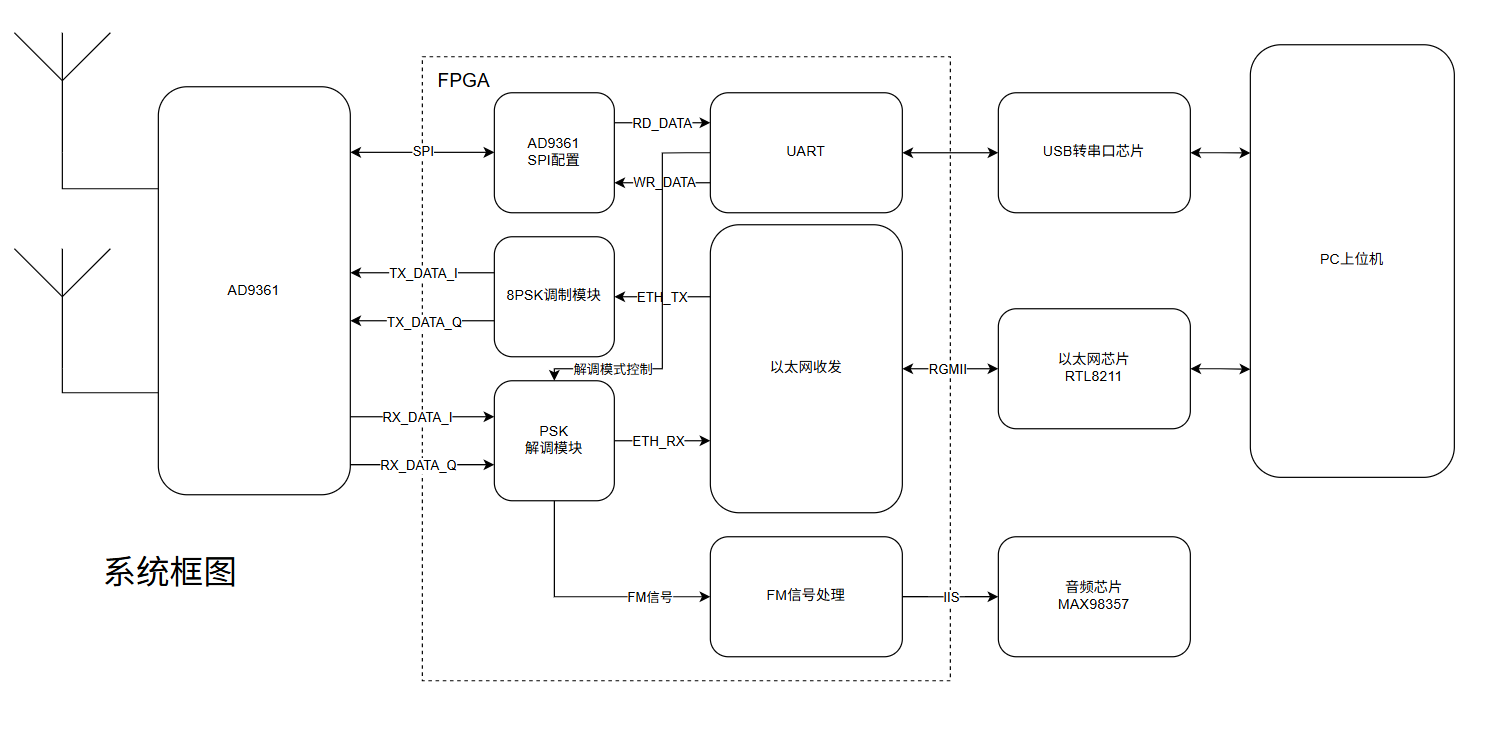
\includegraphics[width=0.8\textwidth]{picture/FPGA/系统整体框图.png}
    \caption{系统整体框图}
    \label{fig:系统整体框图}
\end{figure}

FPGA系统包括AD9361配置模块、UART通信模块、调制解调模块、信号处理模块等。接收通道中，FPGA接收来自AD9361的基带I/Q数据，经过滤波、同步、解调等处理后得到原始信号，随后通过以太网发送到上位机进行进一步处理和分析。发送通道中，FPGA接收上位机发送的数据，经过编码、调制等处理后将数据转换为基带I/Q信号，并通过AD9361进行无线传输。系统的以太网收发依赖于GOWIN Triple Speed Ethernet MAC IP Core与以太网芯片RTL8211，FPGA设计将数据转换为了以太网数据包格式，通过IP核和物理芯片实现了以太网收发。

\subsubsection{AD9361模块}
AD9361模块完成了AD9361的初始化、输入输出差分数据处理、AD9361寄存器读写等功能。AD9361模块通过SPI接口与AD9361进行通信，完成对AD9361寄存器的配置和控制。AD9361模块还包括数据接口部分，负责将来自AD9361的基带I/Q数据进行处理，并将处理后的数据传输到FPGA的其他模块进行后续处理。

\begin{figure}[H]
    \centering
    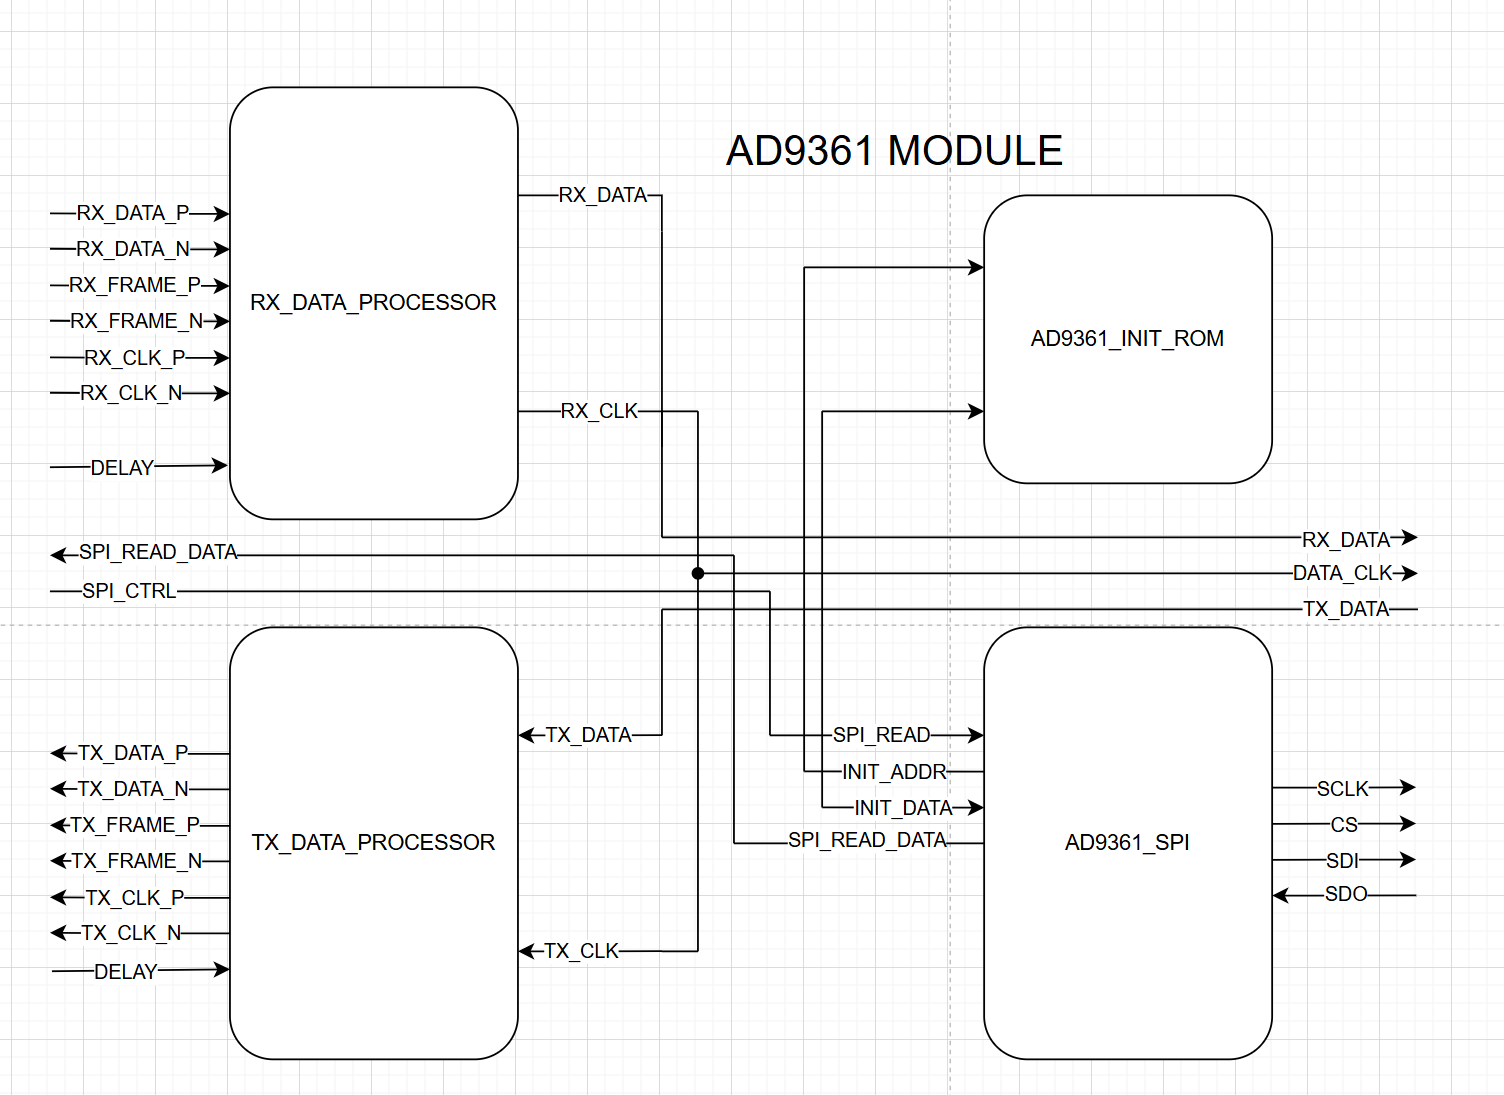
\includegraphics[width=0.8\textwidth]{picture/FPGA/AD9361 module.png}
    \caption{AD9361模块框图}
    \label{fig:AD9361模块框图}
\end{figure}

在该模块中，主要包括以下几个子模块：RX DATA PROCESSOR、TX DATA PROCESSOR、AD9361 SPI和AD9361 INIT ROM。在上电后，AD9361 SPI会首先将AD9361 INIT ROM中的寄存器写入AD9361完成初始化，在初始化结束后，AD9361 SPI会进入待机状态，等待外部信号SPI CTRL来触发SPI的读/写使能状态机，完成对AD9361寄存器的读写操作。读取命令和写入命令来自系统上位机，每次读取会读取AD9361的所有寄存器并发送给上位机，写入命令则会将上位机发送的寄存器地址和数据写入AD9361。

在数据处理部分，RX DATA PROCESSOR负责对来自AD9361的接收数据进行处理，首先利用原语TLVDS IBUF将差分信号转化为单端信号，随后对信号进行延迟处理，延迟量可由上位机实时控制。在数据、数据帧、时钟三者对其后，根据数据帧进行LVDS数据的拼接，最后得到AD9361采集的12位信号和数据时钟。此数据时钟作为后续所有数据处理模块的时钟源。

TX DATA PROCESSOR则负责对发送数据进行处理，输入数据为调制模块输出的基带I/Q数据，根据AD9361 LVDS模式的时序将其拆解为两个6位DDR数据，并且在同时钟下产生数据帧信号。在这种情况下输出的数据、数据帧和数据时钟理论上是对其的，但由于线路延时等问题，实际情况并非如此，因此在TX DATA PROCESSOR中同样加入了IODELAY原语对数据进行延时处理，延迟量同样可由上位机实时控制，确保数据、数据帧和时钟三者对其后发送给AD9361。在数据延迟后，数据、数据帧、数据时钟被TLVDS OBUF转换为差分信号，输出给AD9361。

\subsubsection{UART通信模块}

UART通信模块负责与上位机进行通信，接收上位机发送的指令并将其传输给FPGA的其他模块，同时将FPGA的状态信息发送给上位机。UART通信模块采用标准的UART协议，支持可配置的波特率和数据格式。UART通信模块包括接收、发送和命令处理三个子模块，接收模块负责接收上位机发送的数据，并将数据送入命令集模块转化为相应指令；发送模块负责将AD9361的状态信息等发送给上位机。

\begin{figure}[H]
    \centering
    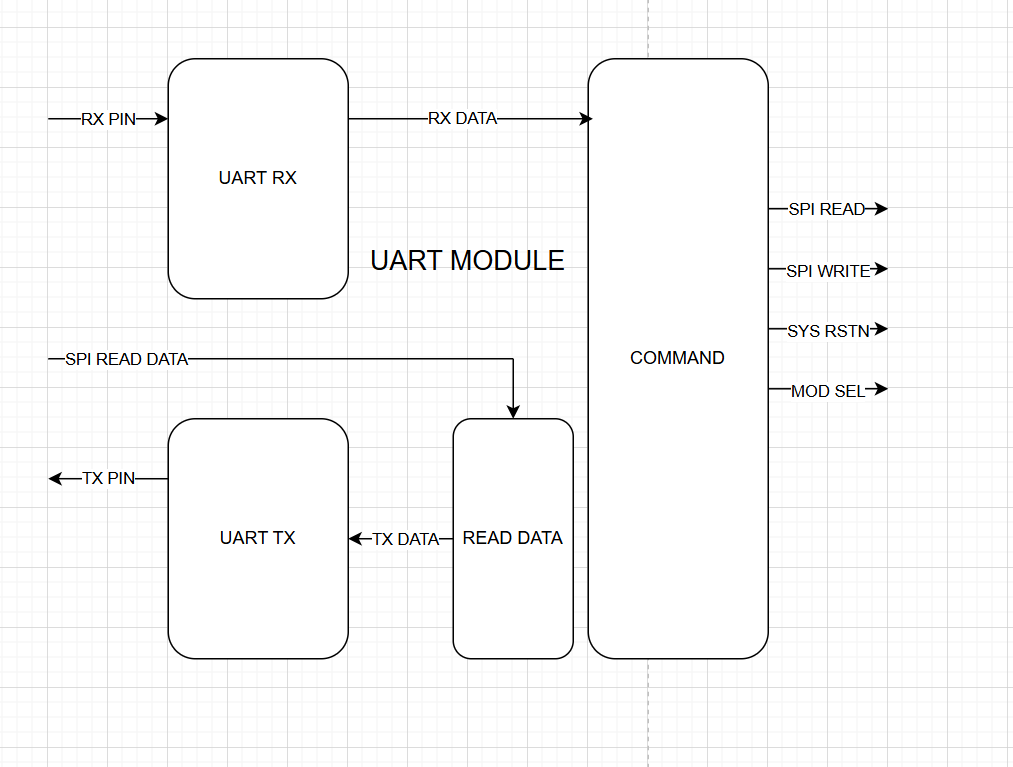
\includegraphics[width=0.8\textwidth]{picture/FPGA/UART module.png}
    \caption{UART通信模块框图}
    \label{fig:UART通信模块框图}
\end{figure}

由于AD9361的寄存器为20位，但是只是用了其中的18位，因此多出的两位就会被浪费掉（这是由于上位机与FPGA之间交互使用了ASCII码，而五个ASCII码在经过转换后为20位）。所以使用余下的两位可以构建寄存器表拓展使用。以此为基础，我们构建了配置本作品各项参数的寄存器表，如下所示：

\begin{figure}[H]
    \centering
    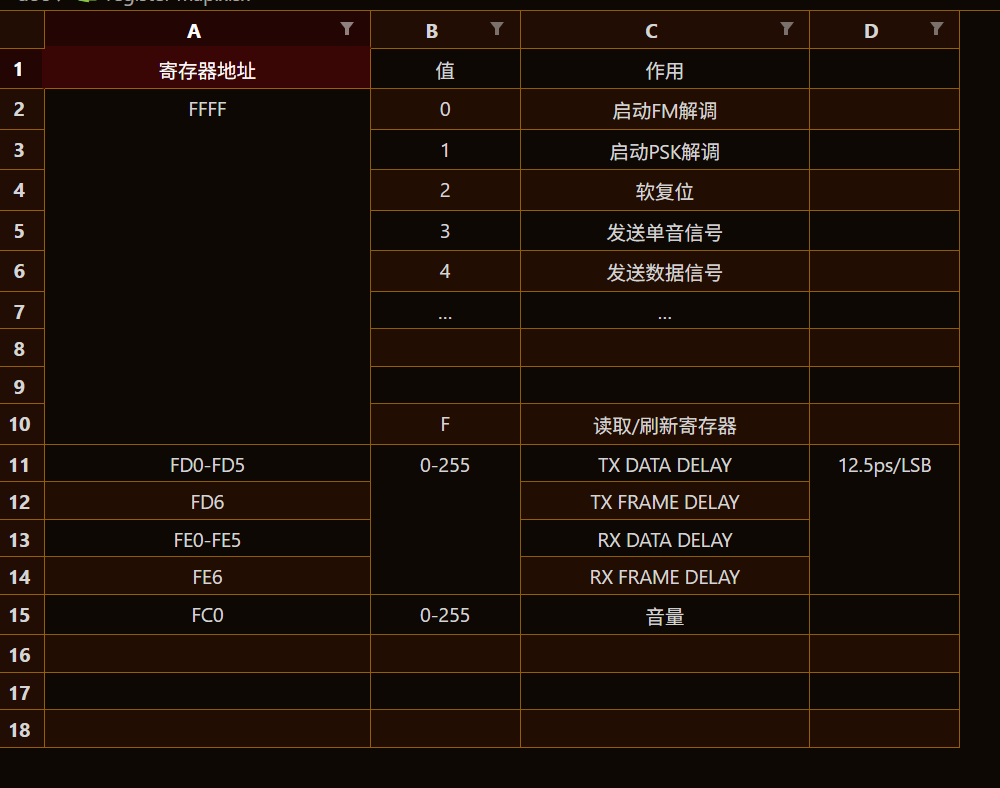
\includegraphics[width=0.8\textwidth]{picture/FPGA/寄存器表.png}
    \caption{UART指令集}
    \label{fig:UART指令集}
\end{figure}

本寄存器表中地址和数据位数并不固定，一方面是为了让出AD9361的寄存器；在另一方面，本作品的寄存器数量少，因此可以通过地址和数据位的灵活配置来实现更多的功能。通过本寄存器表，我们实现了上位机对整体系统的控制。

\subsubsection{调制模块}

本作品使用8PSK调制方式传输数据。调制模块包括输入fifo、8-3转换器和psk调制模块，将以太网输入数据进行8PSK调制，输出基带I/Q数据供TX DATA PROCESSOR使用。

\begin{figure}[H]
    \centering
    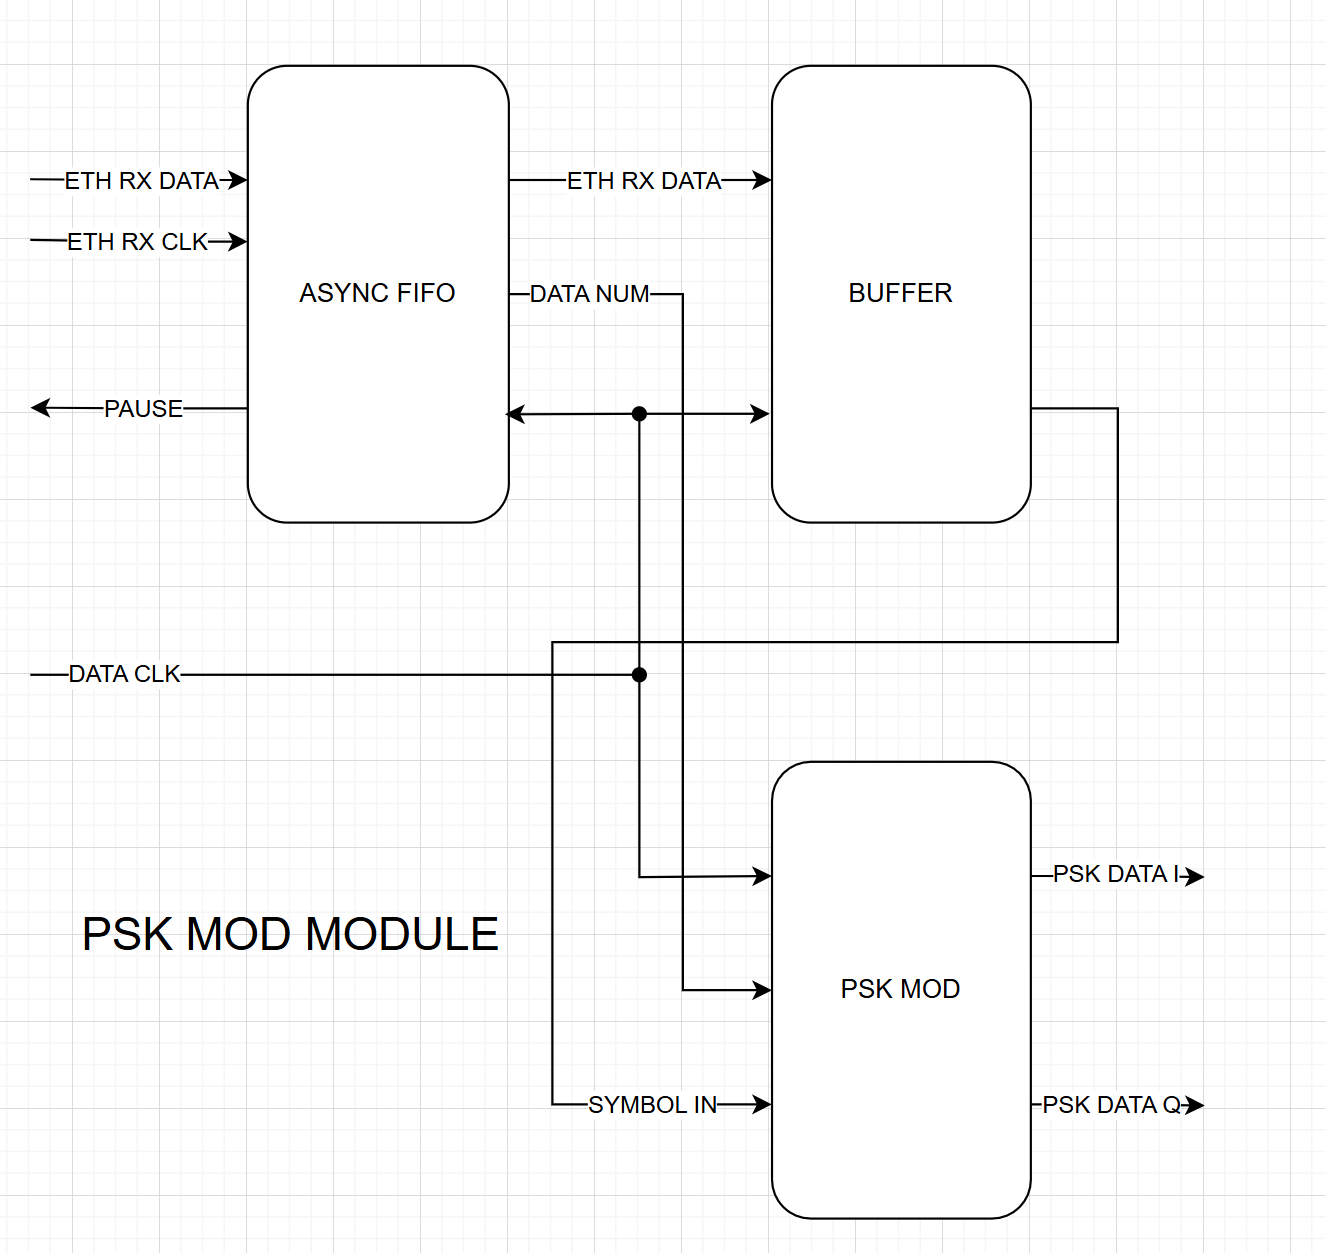
\includegraphics[width=0.8\textwidth]{picture/FPGA/PSK module.png}
    \caption{调制模块框图}
    \label{fig:调制模块框图}
\end{figure}

输入fifo用于缓存以太网输入数据，确保数据的连续性和稳定性。由于射频前端的带宽限制以及调制方式传输速率限制，本作品传输速率最高为30.72Mbps，相比于以太网的传输速率要低很多，因此需要使用fifo对数据进行缓存，防止数据丢失。在输入数据较多时，ASYNC FIFO模块还会输出一个pause信号，来告诉上位机暂停发送数据，防止fifo溢出。在以太网一帧数据全部存入fifo后，buffer会开始将fifo中的数据取出，将8bit数据转换为3bit数据输出。

在数据流通过上述模块后，数据从百兆网数据转换为data clk时钟域下的3bit序列。该序列进入PSK MOD模块进行8PSK调制，该模块使用差分编码方式进行调制，同时也为数据增加了数据帧头和帧尾，方便接收端判断数据是否开始/结束。另一方面，在输出基带I/Q数据时，PSK调制也可以通过调整绝对幅值来控制输出数据幅度的大小，但本作品的射频前端已经能提供接近-90dB的衰减，所以本作品并未采取此种方案，而是选择使用AD9361的衰减模式。

\subsubsection{PSK解调模块}

PSK解调模块负责对接收的基带I/Q数据进行8PSK解调，恢复出原始的数据信号。PSK解调模块包括数据流控部分和解调部分，数据流控部分主要负责对接收的数据进行缓存和同步，确保数据的连续性和正确性。解调部分则负责对缓存后的数据进行8PSK解调，恢复出原始的数据信号。

\begin{figure}[H]
    \centering
    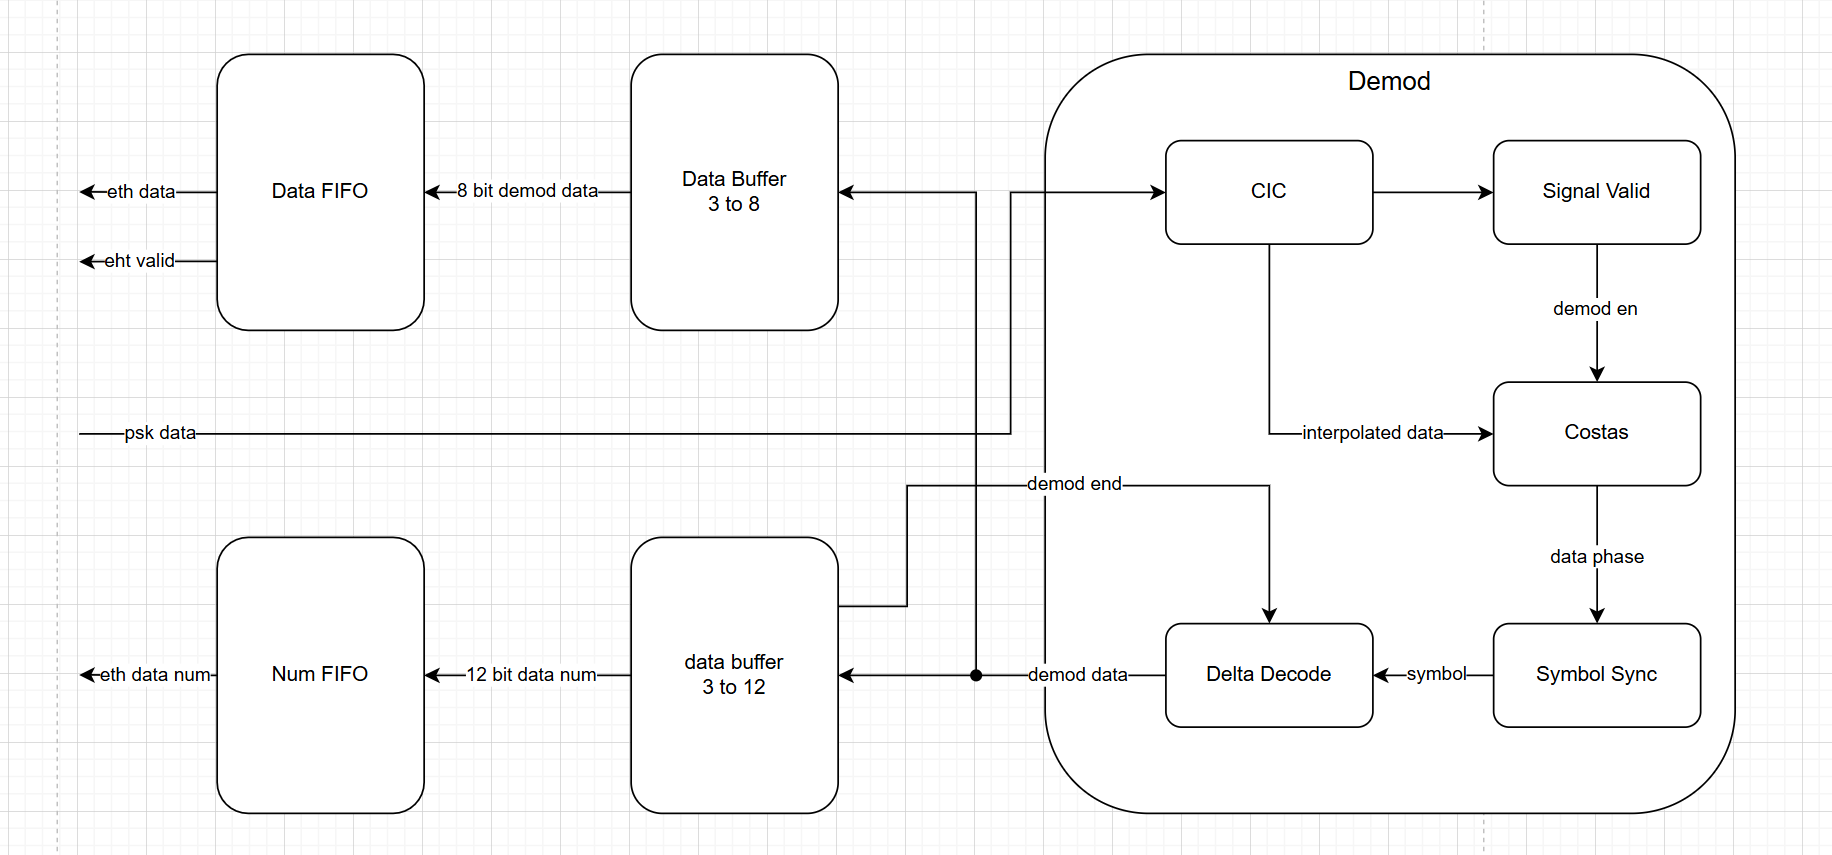
\includegraphics[width=0.8\textwidth]{picture/FPGA/demod module.png}
    \caption{PSK解调模块框图}
    \label{fig:PSK解调模块框图}
\end{figure}

在解调模块，数据首先进入cic内插滤波器滤波，随后在Signal Valid模块对滤波后的信号进行有效判断，有效判断的逻辑是取出滤波后信号的直流分量、交流分量和信号幅值，然后分别设置数个阈值，信号幅值大于其阈值，直流分量大于其阈值且交流分量小于其阈值的时候，判断信号为有效，此时信号开始解调；当信号的幅度小于其阈值时，判断为信号无效，解调帧结束。

在信号有效期间，信号进入PSK DEMOD模块进行8PSK解调。内插信号首先经过costas环进行载波同步，在载波同步锁住信号频偏后，信号的相位被输出并进入符号判决模块进行符号判决。

\subsubsection{FM信号处理模块}
在FM解调模式，解调信号不会通过网口发送至PC上位机，而是通过FPGA内的FM信号处理模块产生IIS音频信号，送至音频解码芯片进行解码播放。FM信号处理模块包括FM解调模块、IIS接口模块和PWM输出模块。
\begin{figure}[H]
    \centering
    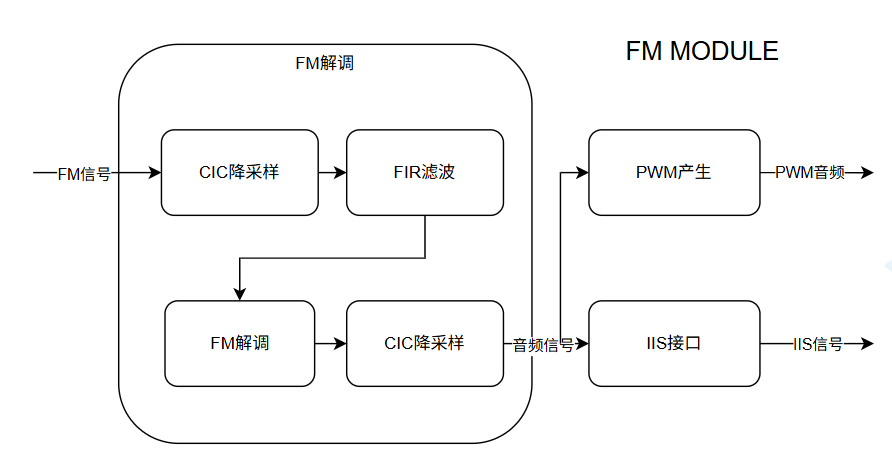
\includegraphics[width=0.8\textwidth]{picture/FPGA/FM module.png}
    \caption{FM信号处理模块框图}
    \label{fig:FM信号处理模块框图}
\end{figure}

FM解调模块首先对输入的原始IQ信号进行CIC降采样、FIR滤波，然后进行FM解调。依据差分解调公式：
\begin{equation*}
    y[n-1] = i[n-1] \cdot q[n] - Q[n-1] \cdot i[n]
\end{equation*}
其中i[n]和q[n]分别为输入的I、Q信号，y[n]为解调后的音频信号。

即可对输入的IQ FM信号进行解调。随后对解调后的音频信号进行低通滤波，滤除高频噪声，得到干净的音频信号。

在对FM信号进行解调后，音频信号会送入IIS接口模块和PWM输出模块进行格式转换。在IIS接口模块，音频信号被转换为IIS格式，并通过IIS接口输出给音频芯片，音频芯片将声音信号解码并通过喇叭播放出来。为了兼容非IIS音频接口，本作品还设置了PWM输出模块，将音频信号转换为PWM信号输出，供非IIS音频芯片使用。

在PWM信号转换模块中，本作品创新性的采用了反序列阈值检测处理，对输出PWM信号进行平均化，降低PWM信号的高频噪声对音质的影响，提高音频播放质量。对于正常的PWM音频输出信号，FPGA根据采样率模拟DAC，将输出信号的幅值作为阈值，使用计数器对PWM信号进行计数，当PWM信号高电平时间大于阈值时，输出高电平，否则输出低电平。但这种方法会使得PWM信号中高频噪声直接影响音质。为此，本作品采用了反序列阈值检测处理，对PWM信号进行平均化处理。具体做法是，FPGA对计数器取反序列，例如三位计数器000、001、010、011、100、101、110、111，取反序列后变为000、100、010、110、001、101、011、111，将反序列与阈值做比较，输出PWM信号，这样能够在保持占空比不变的情况下减少PWM信号中的高频噪声。

\begin{figure}[H]
    \centering
    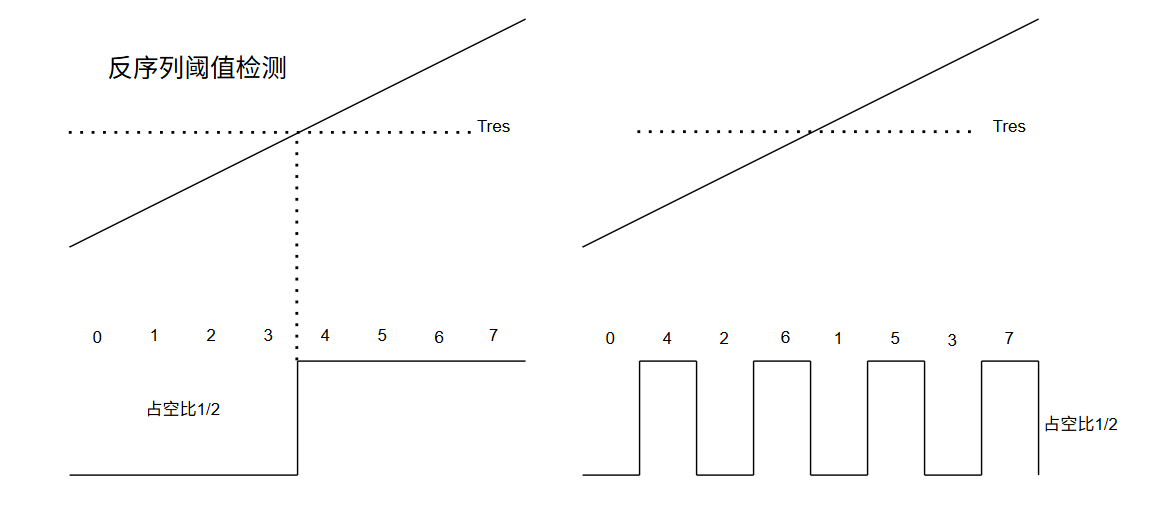
\includegraphics[width=0.8\textwidth]{picture/FPGA/反序列阈值检测.png}
    \caption{反序列阈值检测}
    \label{fig:反序列阈值检测}
\end{figure}

\subsubsection{兼容性设计}

本作品设计兼容TANG MEGA 138K和TANG MEGA 60K。这两款芯片在封装上相似，引脚位置大部分相同，本作品在设计时充分考虑了两款芯片的差异，确保设计能够在两款芯片上顺利运行。主要的兼容性设计包括：
\begin{itemize}[leftmargin=*]
    \item 引脚配置：在设计时，仔细检查两款芯片的引脚分配，确保所有连接均符合两款芯片的要求。对于存在差异的引脚，设计了可配置的引脚映射，以适应不同芯片的需求。确保同一份cst文件可以适用于两款芯片。
    \item 资源利用：考虑到两款芯片在逻辑资源和存储资源上的差异，设计时优化了资源的使用，确保在资源较少的TANG MEGA 60K上也能顺利运行。
    \item 时钟管理：两款芯片可能在时钟管理上存在差异，设计时采用了灵活的时钟管理方案，确保在不同芯片上都能实现稳定的时钟信号。
    \item 测试与验证：在设计完成后，分别在TANG MEGA 138K和TANG MEGA 60K上进行了全面的测试和验证，确保功能和性能均符合预期。
\end{itemize}

\subsection{系统上位机}
\subsubsection{配置上位机}
本作品上位机使用Python QT库开发，提供友好的图形用户界面，方便用户进行射频参数的配置和系统监控。上位机使用uart与FPGA通信，传输速率可自主调整，最高可达115200波特率。上位机会发送5字节ASCII码指令给FPGA，FPGA接收并解码为相应的指令做出响应。系统上位机的主要功能包括：
\begin{itemize}[leftmargin=*]
    \item 射频参数配置：用户可以通过图形界面方便地设置AD9361的工作频率、增益等参数，实时调整以满足不同的应用需求。
    \item 解调模式切换：支持多种解调模式的选择，如PSK、FM等，用户可以根据实际需求进行切换。
    \item 状态监控：上位机能够显示AD9361的工作状态，包括信号强度、误码率等关键指标，能够手动刷新状态、修改寄存器值等，帮助用户了解系统性能和修改系统参数。
    \item 系统软复位：提供软复位功能，允许用户通过上位机界面重置系统，方便调试和恢复系统状态。
    \item 加载自定义配置文件：支持用户加载预设的AD9361配置文件，快速应用不同的工作参数。
    \item 数据记录与分析：支持将射频参数和状态数据记录到本地文件，便于后续分析和优化系统性能。
    \item 用户友好界面：采用直观的图形界面设计，使用户能够轻松操作，无需深入了解底层硬件细节。
\end{itemize}

\begin{figure}[H]
    \centering
    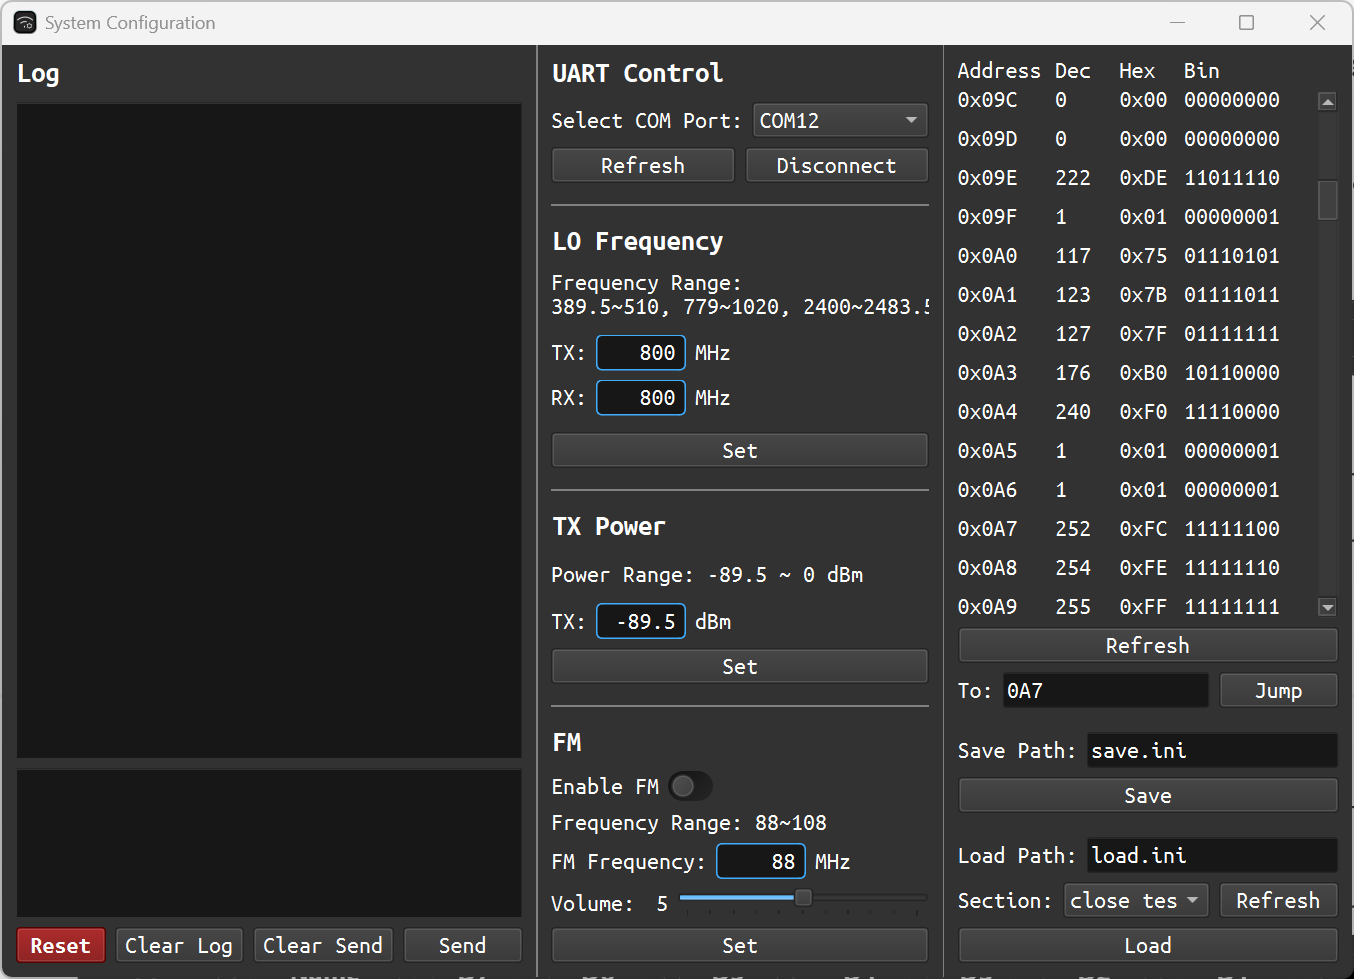
\includegraphics[width=0.8\textwidth]{picture/上位机/上位机界面.png}
    \caption{上位机界面}
    \label{fig:上位机界面}
\end{figure}

上位机主要由三个板块构成，最左侧为消息栏和发送栏，用户可以在消息栏查看系统反馈的信息，在发送栏输入指令并点击SEND即可发送给FPGA，Clear Log和Clear Send分别可以清空消息栏、发送栏的内容，在发送栏的下方还有标红的系统软复位Reset按钮，点击即可进行系统软复位；

中间部分为参数配置区，其中各个板块的作用如下：
\begin{itemize}
    \item UART Control：设置连接的串口，点击Refresh可以刷新串口列表，点击Connect和Disconnect可以连接/断开串口。
    \item LO Frequency：分别设置TX和RX的频率，需要注意的是超出题目范围的LO频率是不可设置的。
    \item TX Power：设置发射功率。
    \item FM：设置是否开启FM解调、FM信号频率以及音频喇叭的音量。
\end{itemize}
需要注意的是：所有设置均需要点击set后才会生效；

右侧为状态监控区，在板卡上电后，系统会将AD9361的所有寄存器读取并显示在状态监控区，用户可以通过点击Refresh手动刷新寄存器状态，Refresh下方的Jump按钮可以快速跳转到指定的寄存器位置。在寄存器监控栏内，寄存器内容将会以地址、十进制值、十六进制值和二进制值四种形式显示，用户可以直接双击任意寄存器值对其进行修改，
或者在输入框中输入寄存器地址和数值来修改寄存器的值。在Jump按键的下方，可以选择保存寄存器数据到制定路径。上位机也支持加载预设的寄存器配置文件，用户可以在Load Path中输入文件位置来加载预设的配置文件，点击Refresh即可刷新。例如目前上位机加载的文件load.ini为配置TX、RX延时的寄存器文件，在section中选择rx data test并点击load可以将3f500，3f40b依次写入AD9361，点击set rx delay可以将设置的7个延时数据依次加载入FPGA中的RX IODELAY原语中。.ini文件中的数据格式如下图。

\begin{figure} [H] 
    \centering
    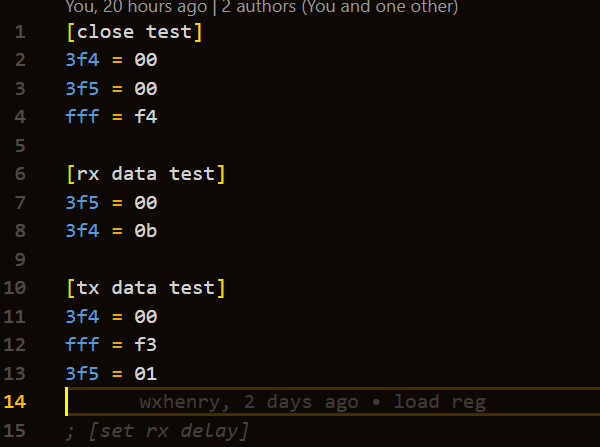
\includegraphics[width=0.6\textwidth]{picture/上位机/ini文件内容格式.png}
    \caption{ini文件内容格式}
    \label{fig:ini文件内容格式}
\end{figure}

需要指出的是，所有的配置都可以通过左侧的发送栏发送对应的ASCII码指令来实现，用户可以通过上位机消息栏界面查看对应的指令格式，并通过发送栏发送指令来实现对系统的控制。
\subsubsection{网口上位机}

\subsubsection{Local Send}

\subsection{射频前端}
本作品使用AD9361的官方评估版FMCOMMS3作为射频前端。AD9361是一款高性能、集成度高的RF收发器，支持宽频带和多种调制方式，适用于各种无线通信应用。FMCOMMS3评估板提供了完整的硬件平台，方便用户进行快速原型开发和测试。AD9361包含了射频收发器、模数转换器（ADC）、数模转换器（DAC）以及数字信号处理模块，支持从70 MHz到6 GHz的频率范围，带宽可达56 MHz。该评估板还配备了多种接口，如LVDS、SPI和I2C，便于与FPGA或处理器进行通信。此外，FMCOMMS3评估板具有灵活的配置选项，允许用户根据具体应用需求调整参数，如增益控制、滤波器设置和频率规划。通过使用AD9361和FMCOMMS3评估板，用户能够快速实现高性能的无线通信系统设计，满足不同应用场景的需求。AD9361采用零中频架构直接变频器具有非常优异的噪声系数和线性度，对射频前端的低噪声放大器的要求不高。发射器同样采用直接变频架构，可以满足较高的调制精度，同时拥有超低的噪声特性。

在内部接收信号处理流程中，射频信号通过信号接收通道传送到基带处理器，经过多级滤波器改善其数字信号的信噪比，最后根据配置的不同，I、Q 两路信号会以不同的交织方式组成一路或者两路信号传送给基带处理单元进行后续的数据处理。相比基于分立元件构建的信号特征提取与识别系统，AD9361 采用了高度集成化的设计，具有良好的性能和较低的功耗，不仅能简化系统结构，而且可以避免因射频链路设计缺陷引起的信号调制识别设备性能难以满足系统设计需求的问题。

AD9361含有2个接收通道和2个发送通道，支持TDD和FDD两种工作模式，本作品使用lvds，1R1T，FDD模式。

\begin{figure}[H]
    \centering
    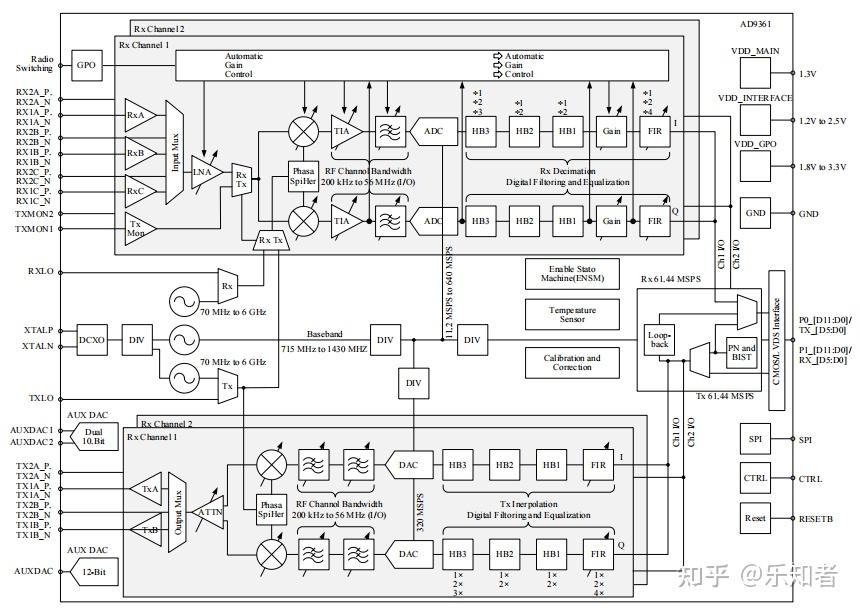
\includegraphics[width=0.8\textwidth]{picture/AD9361/AD9361系统框图.png}
    \caption{AD9361系统框图}
    \label{fig:AD9361系统框图}
\end{figure}

\subsubsection{AD9361配置流程}
AD9361的配置主要是通过调整寄存器的值来进行，AD9361有超过1000个寄存器，每个寄存器都有特定的功能和作用。正确配置AD9361是本作品的关键步骤之一。配置流程主要包括以下几个步骤：
\begin{itemize}[leftmargin=*]
    \item 根据应用需求确定合适的工作模式，重点需要确定频率范围、带宽和增益等参数。
    \item 根据频率范围和带宽选择合适的滤波器设置，利用官方提供的Matlab工具AD936x filter wizard生成滤波器ftr文件。
    \item 使用官方提供的配置工具AD9361 Evaluation Software对AD9361进行初始配置。使用已经确定好的滤波器文件、工作模式和其他参数进行配置，生成初始化寄存器表。
    \item 将寄存器配置转换为verilog代码，方便在FPGA中实现对AD9361的控制。
    \item 上板验证，依次校准通道数据延时、IQ正交校准、DC偏移等参数，确保AD9361工作在最佳状态。最后进行增益配置，根据选择的增益模式进行增益的调整。
\end{itemize}

后续对AD9361配置的介绍中会提到寄存器配置的具体内容，所有提到的寄存器包括其值均为16进制表示，AD9361的寄存器地址范围为0x000到0x3FE，每个寄存器的值为8位。

本题目要求频率可选择 389.5~510.0MHz，779~1020MHz，2400~2483.5MHz 等三个频段中的任意一个，对于AD9351来说，这些频段均在其工作范围之内，可以通过配置寄存器来实现频率的实时切换。作品要求实现数据、语音、视频等信号的无线传输，综合考虑数据速率和传输距离，选择16MHz的带宽、61.44MHz的采样率进行传输。

使用官方Matlab插件AD936x Filter Wizard设计滤波器，分别为TX和RX生成对应的滤波器系数文件。选择正确的采样率和带宽，设计出满足要求的滤波器，并将滤波器系数导出为FTR文件，供后续配置使用。

\begin{figure}[H]
    \centering
    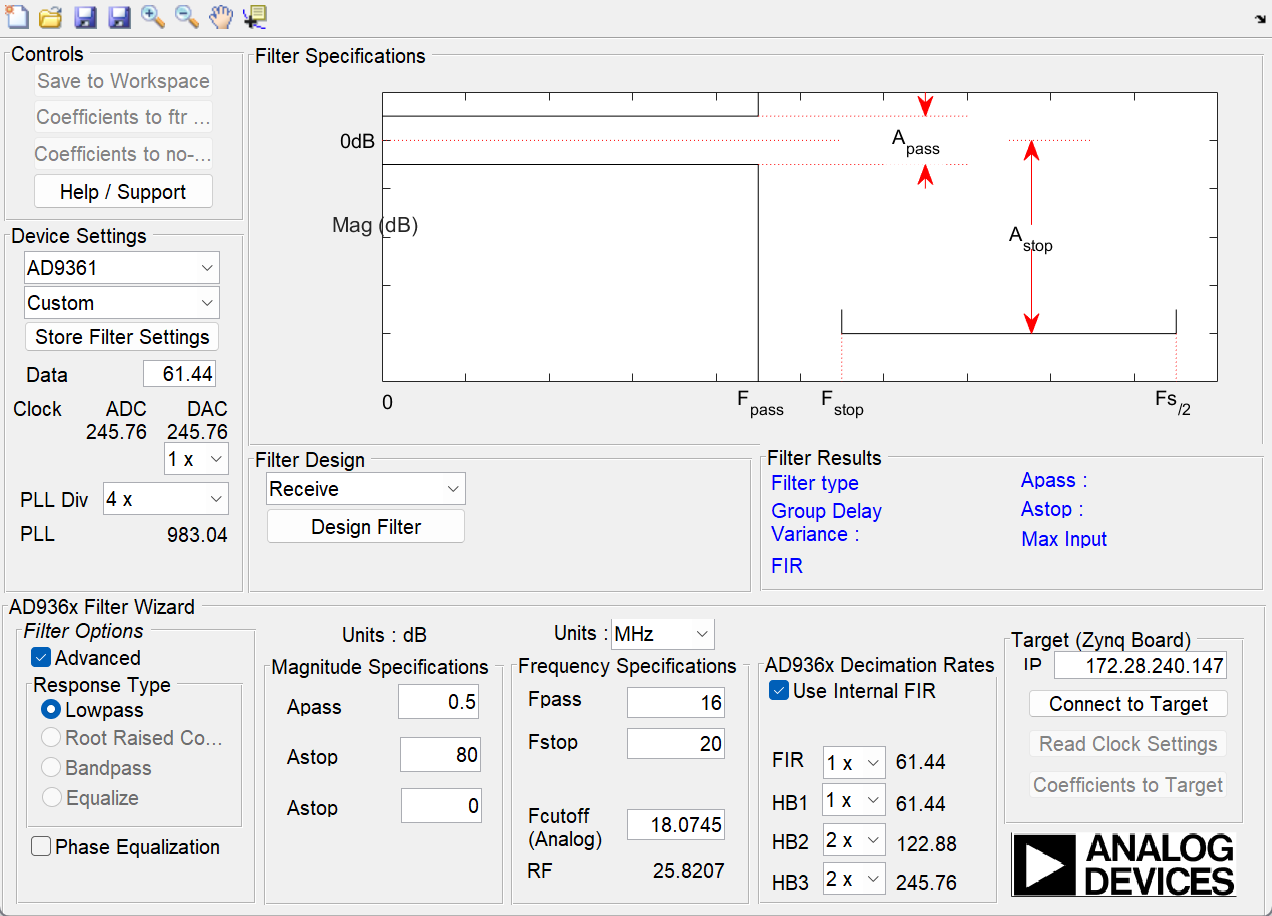
\includegraphics[width=0.8\textwidth]{picture/AD9361/AD9361 filter.png}
    \caption{AD9361滤波器设计工具}
    \label{fig:AD9361滤波器设计工具}
\end{figure}

随后在AD9361 Evaluation Software中进行基本配置。首先在第一页配置器件版本、是否使用模板以及通道数量。

\begin{figure}[H]
    \centering
    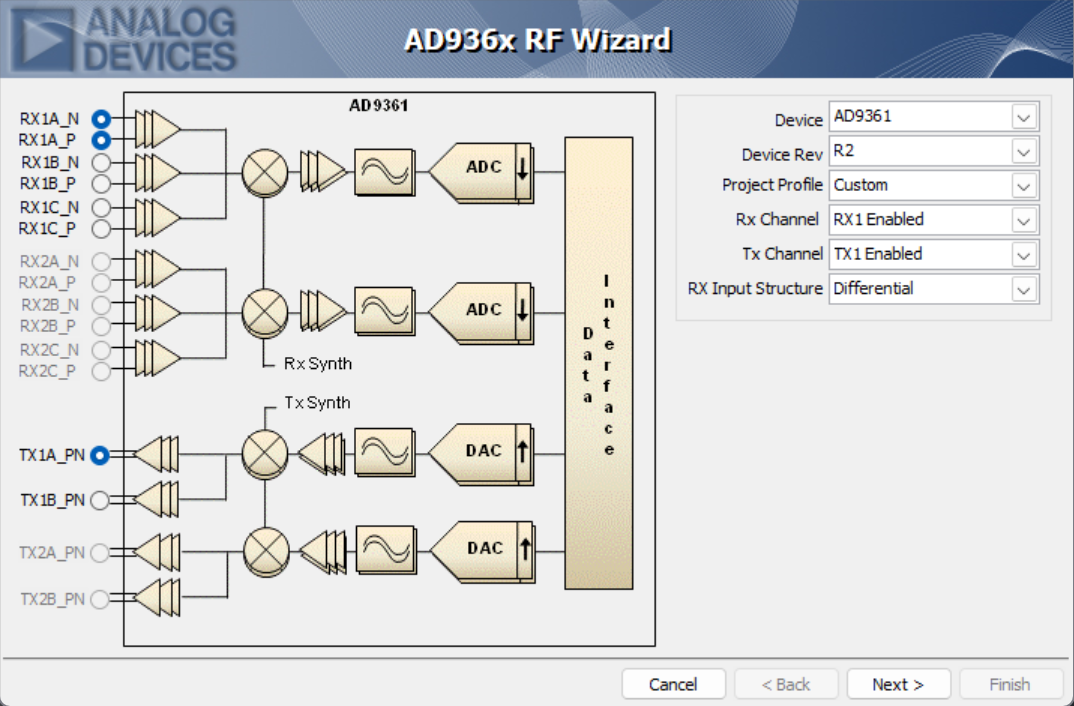
\includegraphics[width=0.8\textwidth]{picture/AD9361/AD9361 基本配置 page1.png}
    \caption{AD9361 Evaluation Software基本配置1}
    \label{fig:AD9361 Evaluation Software基本配置1}
\end{figure}

在第二页配置输入参考时钟来源为外部晶振，频率为40MHz，设置DCXO和PLL参数，确定AD9361的BBPLL和RFPLL的输入频率，以便于以后对LO进行配置。

\begin{figure}[H]
    \centering
    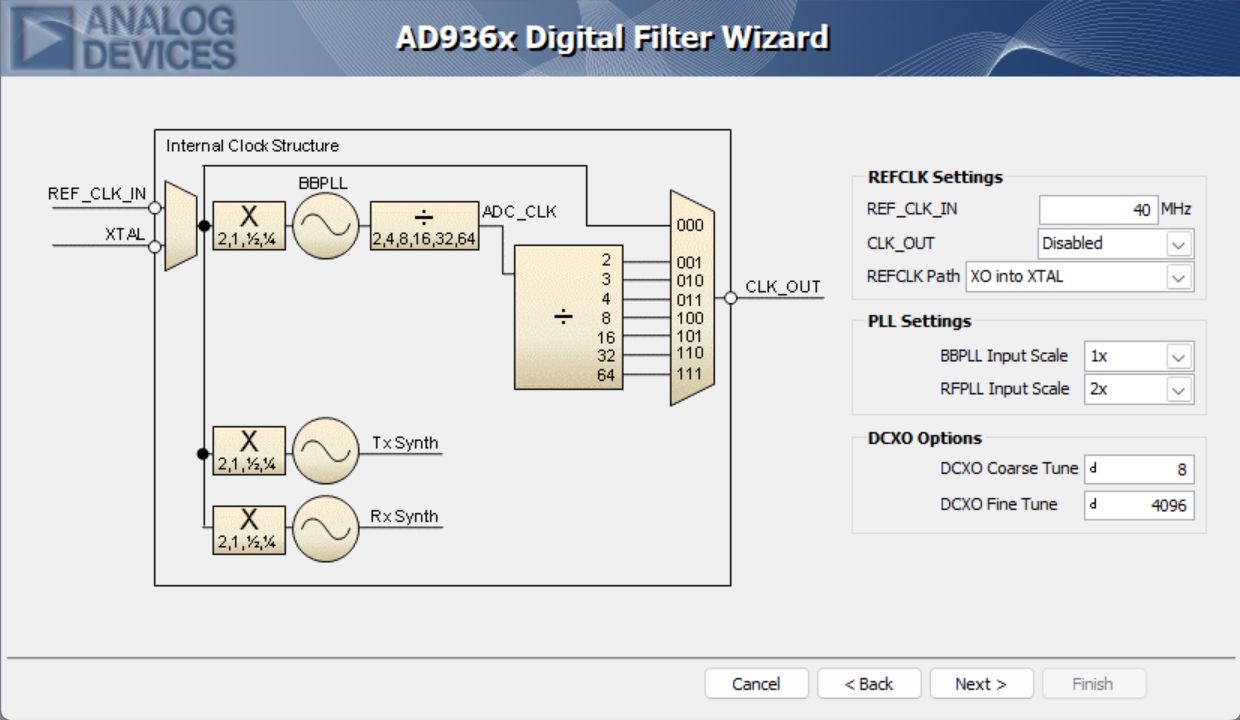
\includegraphics[width=0.8\textwidth]{picture/AD9361/AD9361 基本配置 page2.png}
    \caption{AD9361 Evaluation Software基本配置2}
    \label{fig:AD9361 Evaluation Software基本配置2}
\end{figure}

在第三页配置采样率为61.44MHz，带宽为16MHz，并在第四页和第五页分别为TX、RX选择对应的滤波器文件。

\begin{figure}[H]
    \centering
    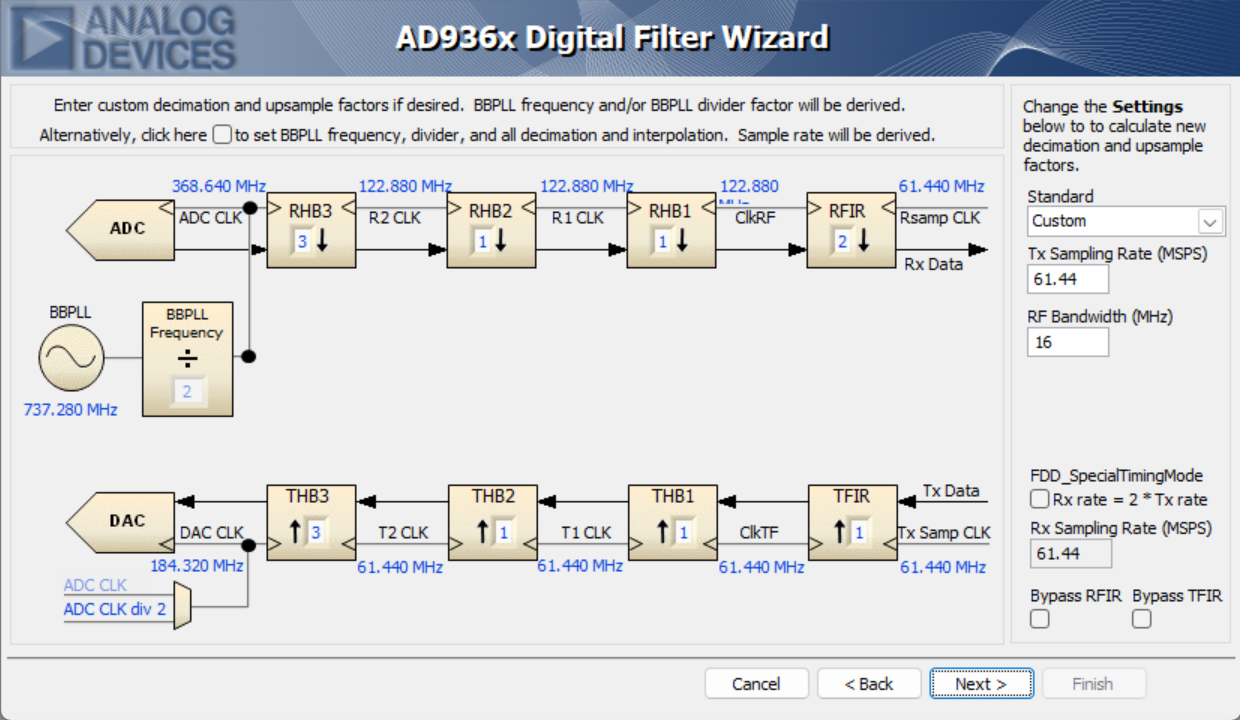
\includegraphics[width=0.8\textwidth]{picture/AD9361/AD9361 基本配置 page3.png}
    \caption{AD9361 Evaluation Software基本配置3}
    \label{fig:AD9361 Evaluation Software基本配置3}
\end{figure}

\begin{figure}[H]
    \centering
    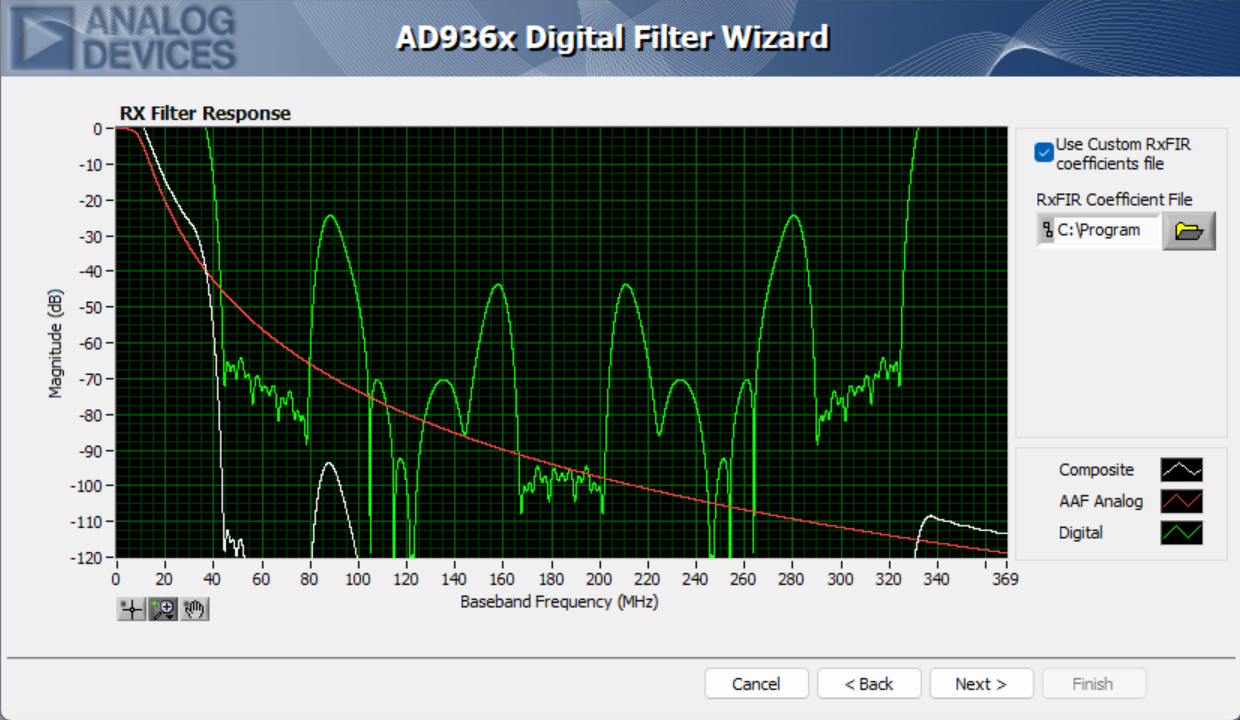
\includegraphics[width=0.8\textwidth]{picture/AD9361/AD9361 基本配置 page4.png}
    \caption{AD9361 Evaluation Software基本配置4}
    \label{fig:AD9361 Evaluation Software基本配置4}
\end{figure}

\begin{figure}[H]
    \centering
    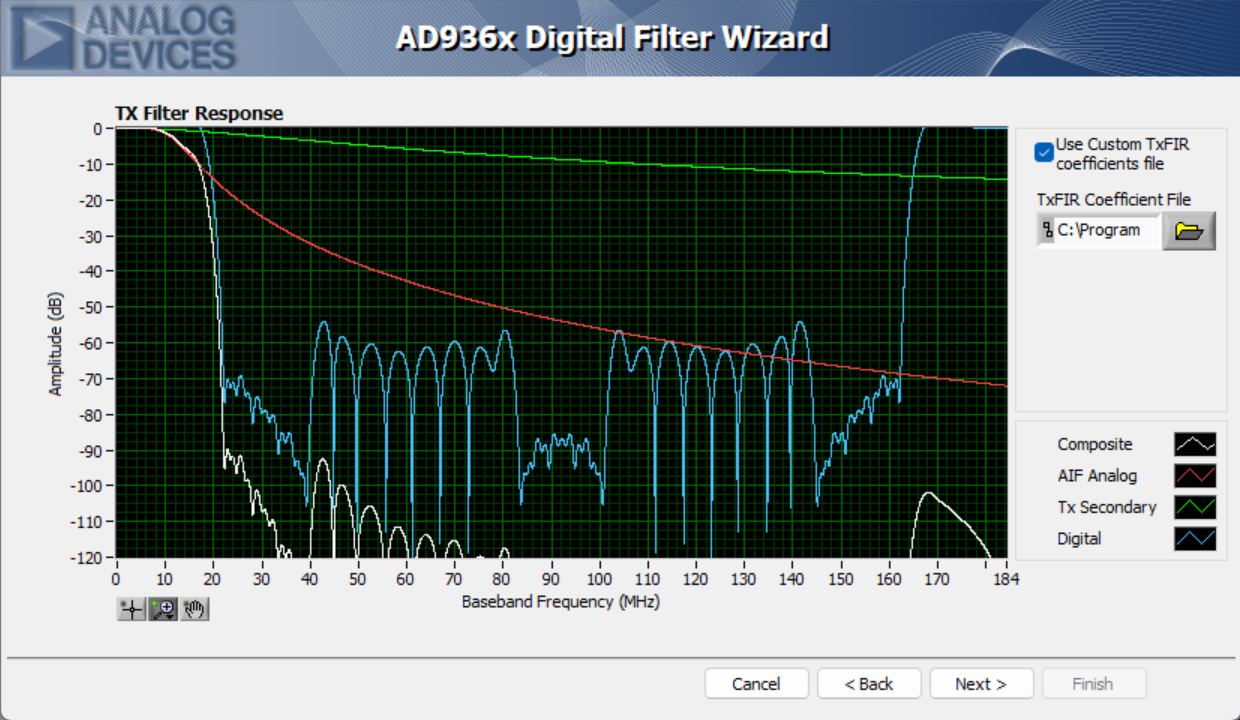
\includegraphics[width=0.8\textwidth]{picture/AD9361/AD9361 基本配置 page5.png}
    \caption{AD9361 Evaluation Software基本配置5}
    \label{fig:AD9361 Evaluation Software基本配置5}
\end{figure}

在第六页选择工作模式为LVDS，FDD。

\begin{figure}[H]
    \centering
    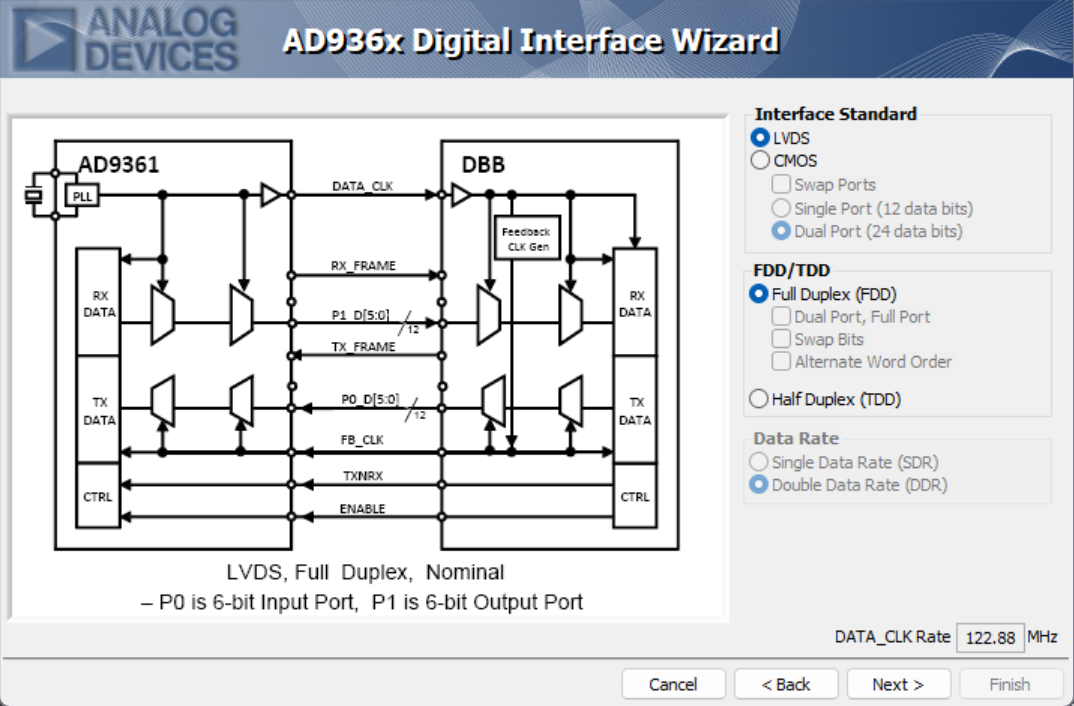
\includegraphics[width=0.8\textwidth]{picture/AD9361/AD9361 基本配置 page6.png}
    \caption{AD9361 Evaluation Software基本配置6}
    \label{fig:AD9361 Evaluation Software基本配置6}
\end{figure}

第七页是选择PN翻转、IQ翻转等设置，本作品在初始化阶段未进行修改。在后续的上板验证中会进行相应的调整。

\begin{figure}[H]
    \centering
    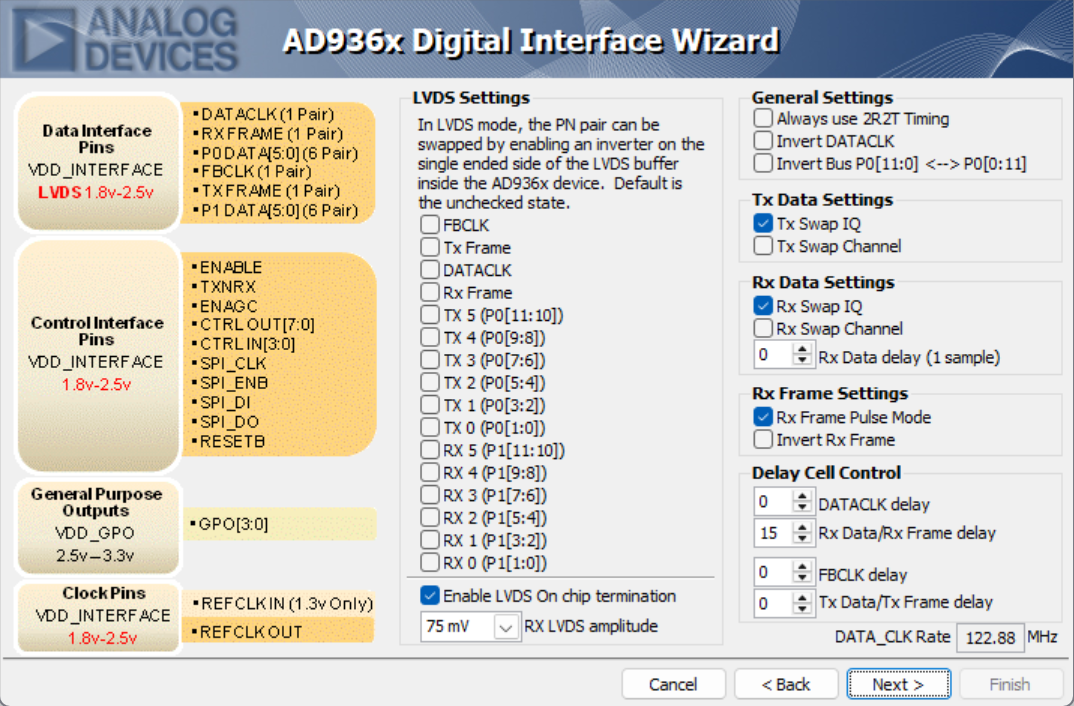
\includegraphics[width=0.8\textwidth]{picture/AD9361/AD9361 基本配置 page7.png}
    \caption{AD9361 Evaluation Software基本配置7}
    \label{fig:AD9361 Evaluation Software基本配置7}
\end{figure}

第八页是ENSM设置，选择FDD和SPI控制模式，SPI控制模式可以更方便的利用上位机对工作状态进行修改，启用ENABLE、TXNRX两个在FDD中的非必要信号对TX、RX通道进行控制，方便实时控制发送与关闭。

\begin{figure}[H]
    \centering
    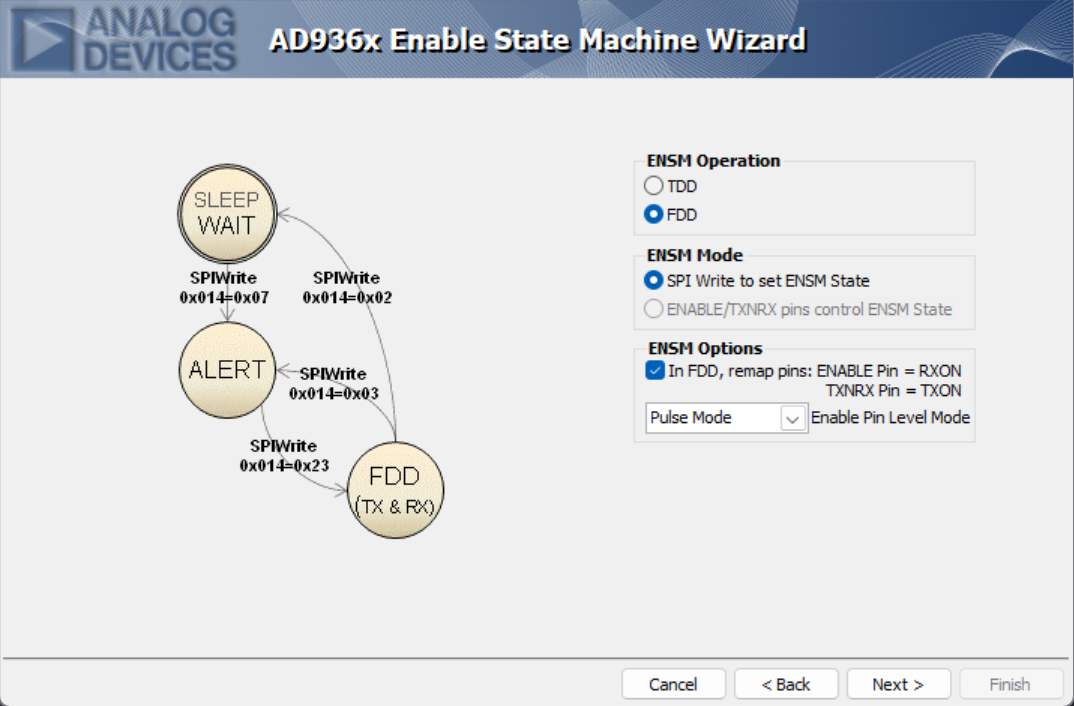
\includegraphics[width=0.8\textwidth]{picture/AD9361/AD9361 基本配置 page8.png}
    \caption{AD9361 Evaluation Software基本配置8}
    \label{fig:AD9361 Evaluation Software基本配置8}
\end{figure}

在最后一页选择AGC模式为FAST ATTACK，点击finish后在首页导出为寄存器配置文本。使用本作品中的Phyton脚本将寄存器文本转换为verilog代码，方便在FPGA中进行调用。

\begin{figure}[H]
    \centering
    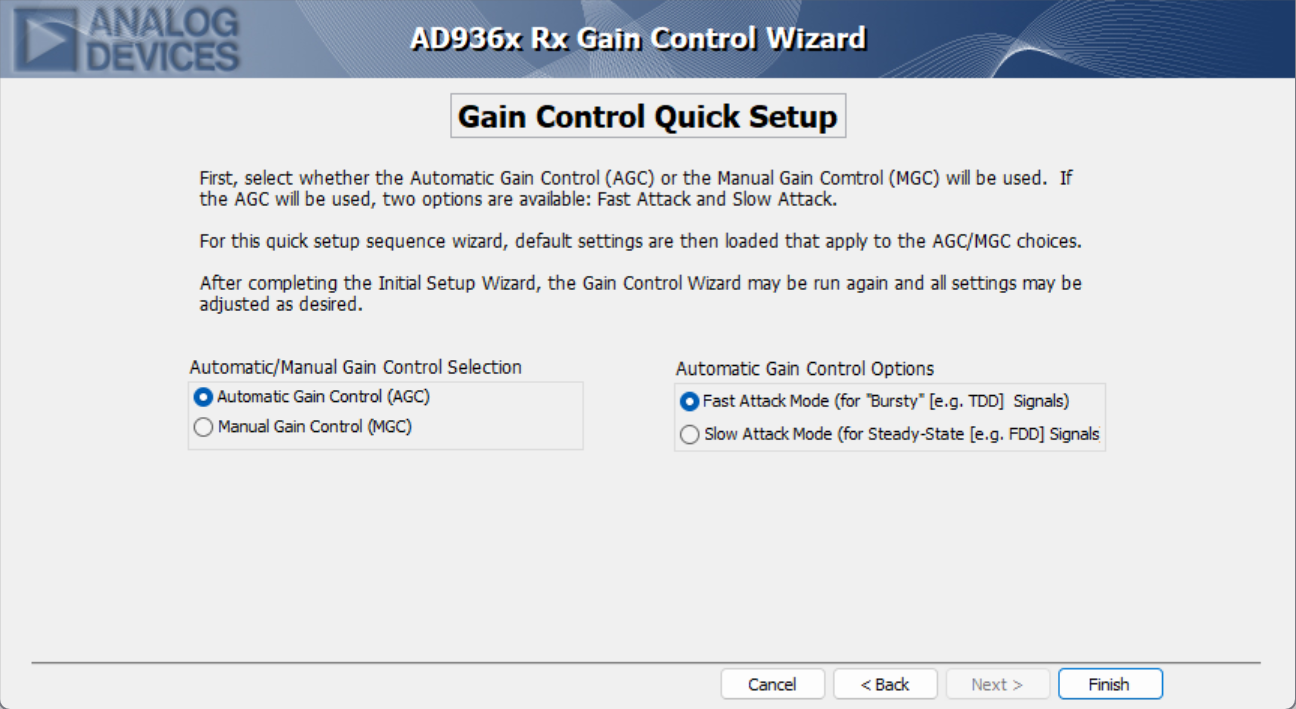
\includegraphics[width=0.8\textwidth]{picture/AD9361/AD9361 基本配置 page9.png}
    \caption{AD9361 Evaluation Software基本配置9}
    \label{fig:AD9361 Evaluation Software基本配置9}
\end{figure}

随后进行上板验证，首先利用3F4-3F5寄存器启动芯片自检，利用006-007寄存器校准通道数据延时。根据官方提供的自检手册，首先设置3F40B，使芯片内部生成一个单音信号直接通给RX接收输出点，不经过内部模拟通道。然后利用gao逻辑分析仪抓取rx数据波形，参考官方提供的数据时序图，时序错误可能会导致数据高低位反拼接，或者IQ翻转拼接并且一路数据反拼接，根据这两种情况对时延进行调整。除去006-007提供0.3ns/LSB的调整外，我们在FPGA内部准备了IODELAY原语对其进行延迟，使用上位机进行配置延迟时间，该原语提供12.5ps/LSB的调整精度，可以更精细的调整时序，最终达到了理想的时序效果。

\begin{figure}[H]
    \centering
    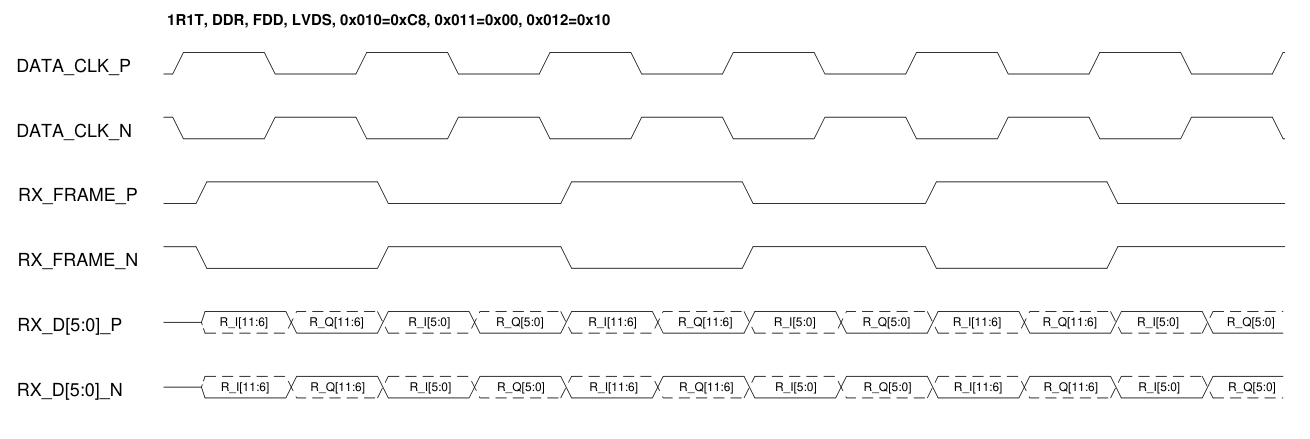
\includegraphics[width=0.8\textwidth]{picture/AD9361/AD9361 RX TIMING.png}
    \caption{AD9361 LVDS 1T1R RX 时序图}
    \label{fig:AD9361 RX 时序图}
\end{figure}

随后设置3F400，3F501启动TX通道校准，在这种设置下，TX接口会被直连至RX接口，在FPGA内产生一个单音信号给TX，就能在RX接口接收到相应的信号，由于目前已经调好RX的时延，RX的时序已经完全正确，所以此时能够对TX进行校准。TX的时序与RX类似，使用相同的调整方法即可。需要注意的是，在调整延时时可能会遇到TX/RX FRAME和DATA错位180°的问题，在这种时候可以通过调整此前已经提到的TX/RX FRAME的PN翻转来解决，相应的寄存器为03D和03E。

\begin{figure}[H]
    \centering
    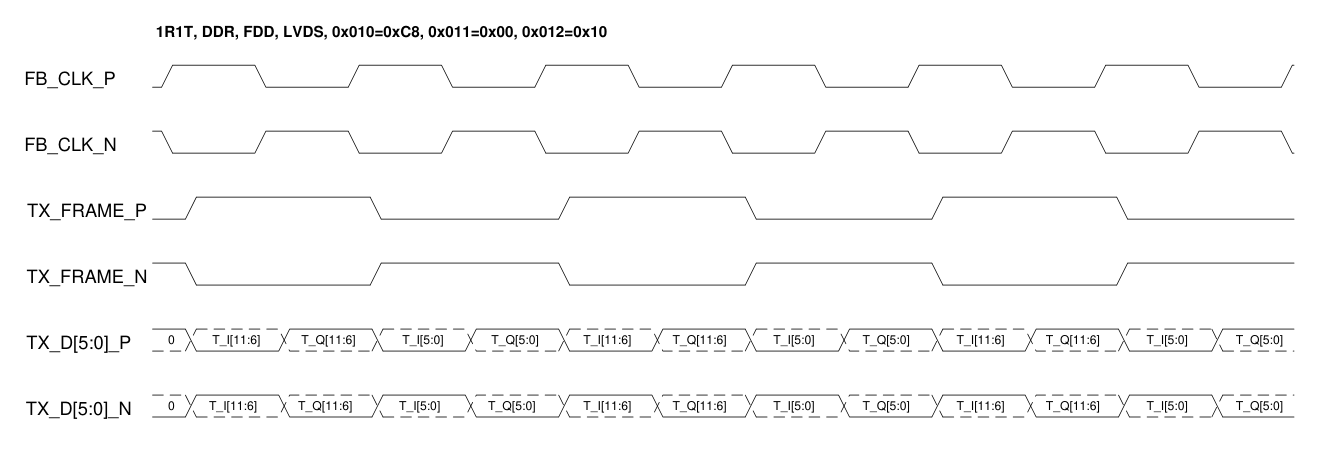
\includegraphics[width=0.8\textwidth]{picture/AD9361/AD9361 TX TIMING.png}
    \caption{AD9361 LVDS 1T1R TX 时序图}
    \label{fig:AD9361 TX 时序图}
\end{figure}

完成时序校准后，进行IQ正交校准和DC偏移的校准。首先进行IQ正交校准，通过设置3F403使用AD9361内部单音信号源，发送一个已知频率的单音信号，单音信号的频率可以通过3F4[7:6]配置，随后通过频谱仪观测TX信号的频谱图。
此时可以观测到TX信号不仅有本振泄露，还有镜像干扰。通过设置09F01，开启手动调整TX Quadrature Calibration功能，然后对08E-08F寄存器进行调整，直到镜像消失。镜像校准后，进行本振泄露校准，调整0A0-0A1寄存器中的NCO频率，直到本振泄露最小。


AD9361具有DC offset tracking功能，可以自动校准DC偏移，但是在连续发送同一个符号时，该功能可能反而会导致DC偏移加重。发送调制信号并且从外部环回RX通道，使用gao抓取波形在上位机分析采样点分布情况，可以看出采样点是否出现DC偏移。先发送不存在连续同符号序列，开启DC offset tracking，观察采样点分布情况，若采样点分布正常，则说明DC offset tracking已经正确校准DC偏移，随后关闭该功能即可。

\begin{figure} [H]
    \centering
    % 逆时针旋转 90 度
    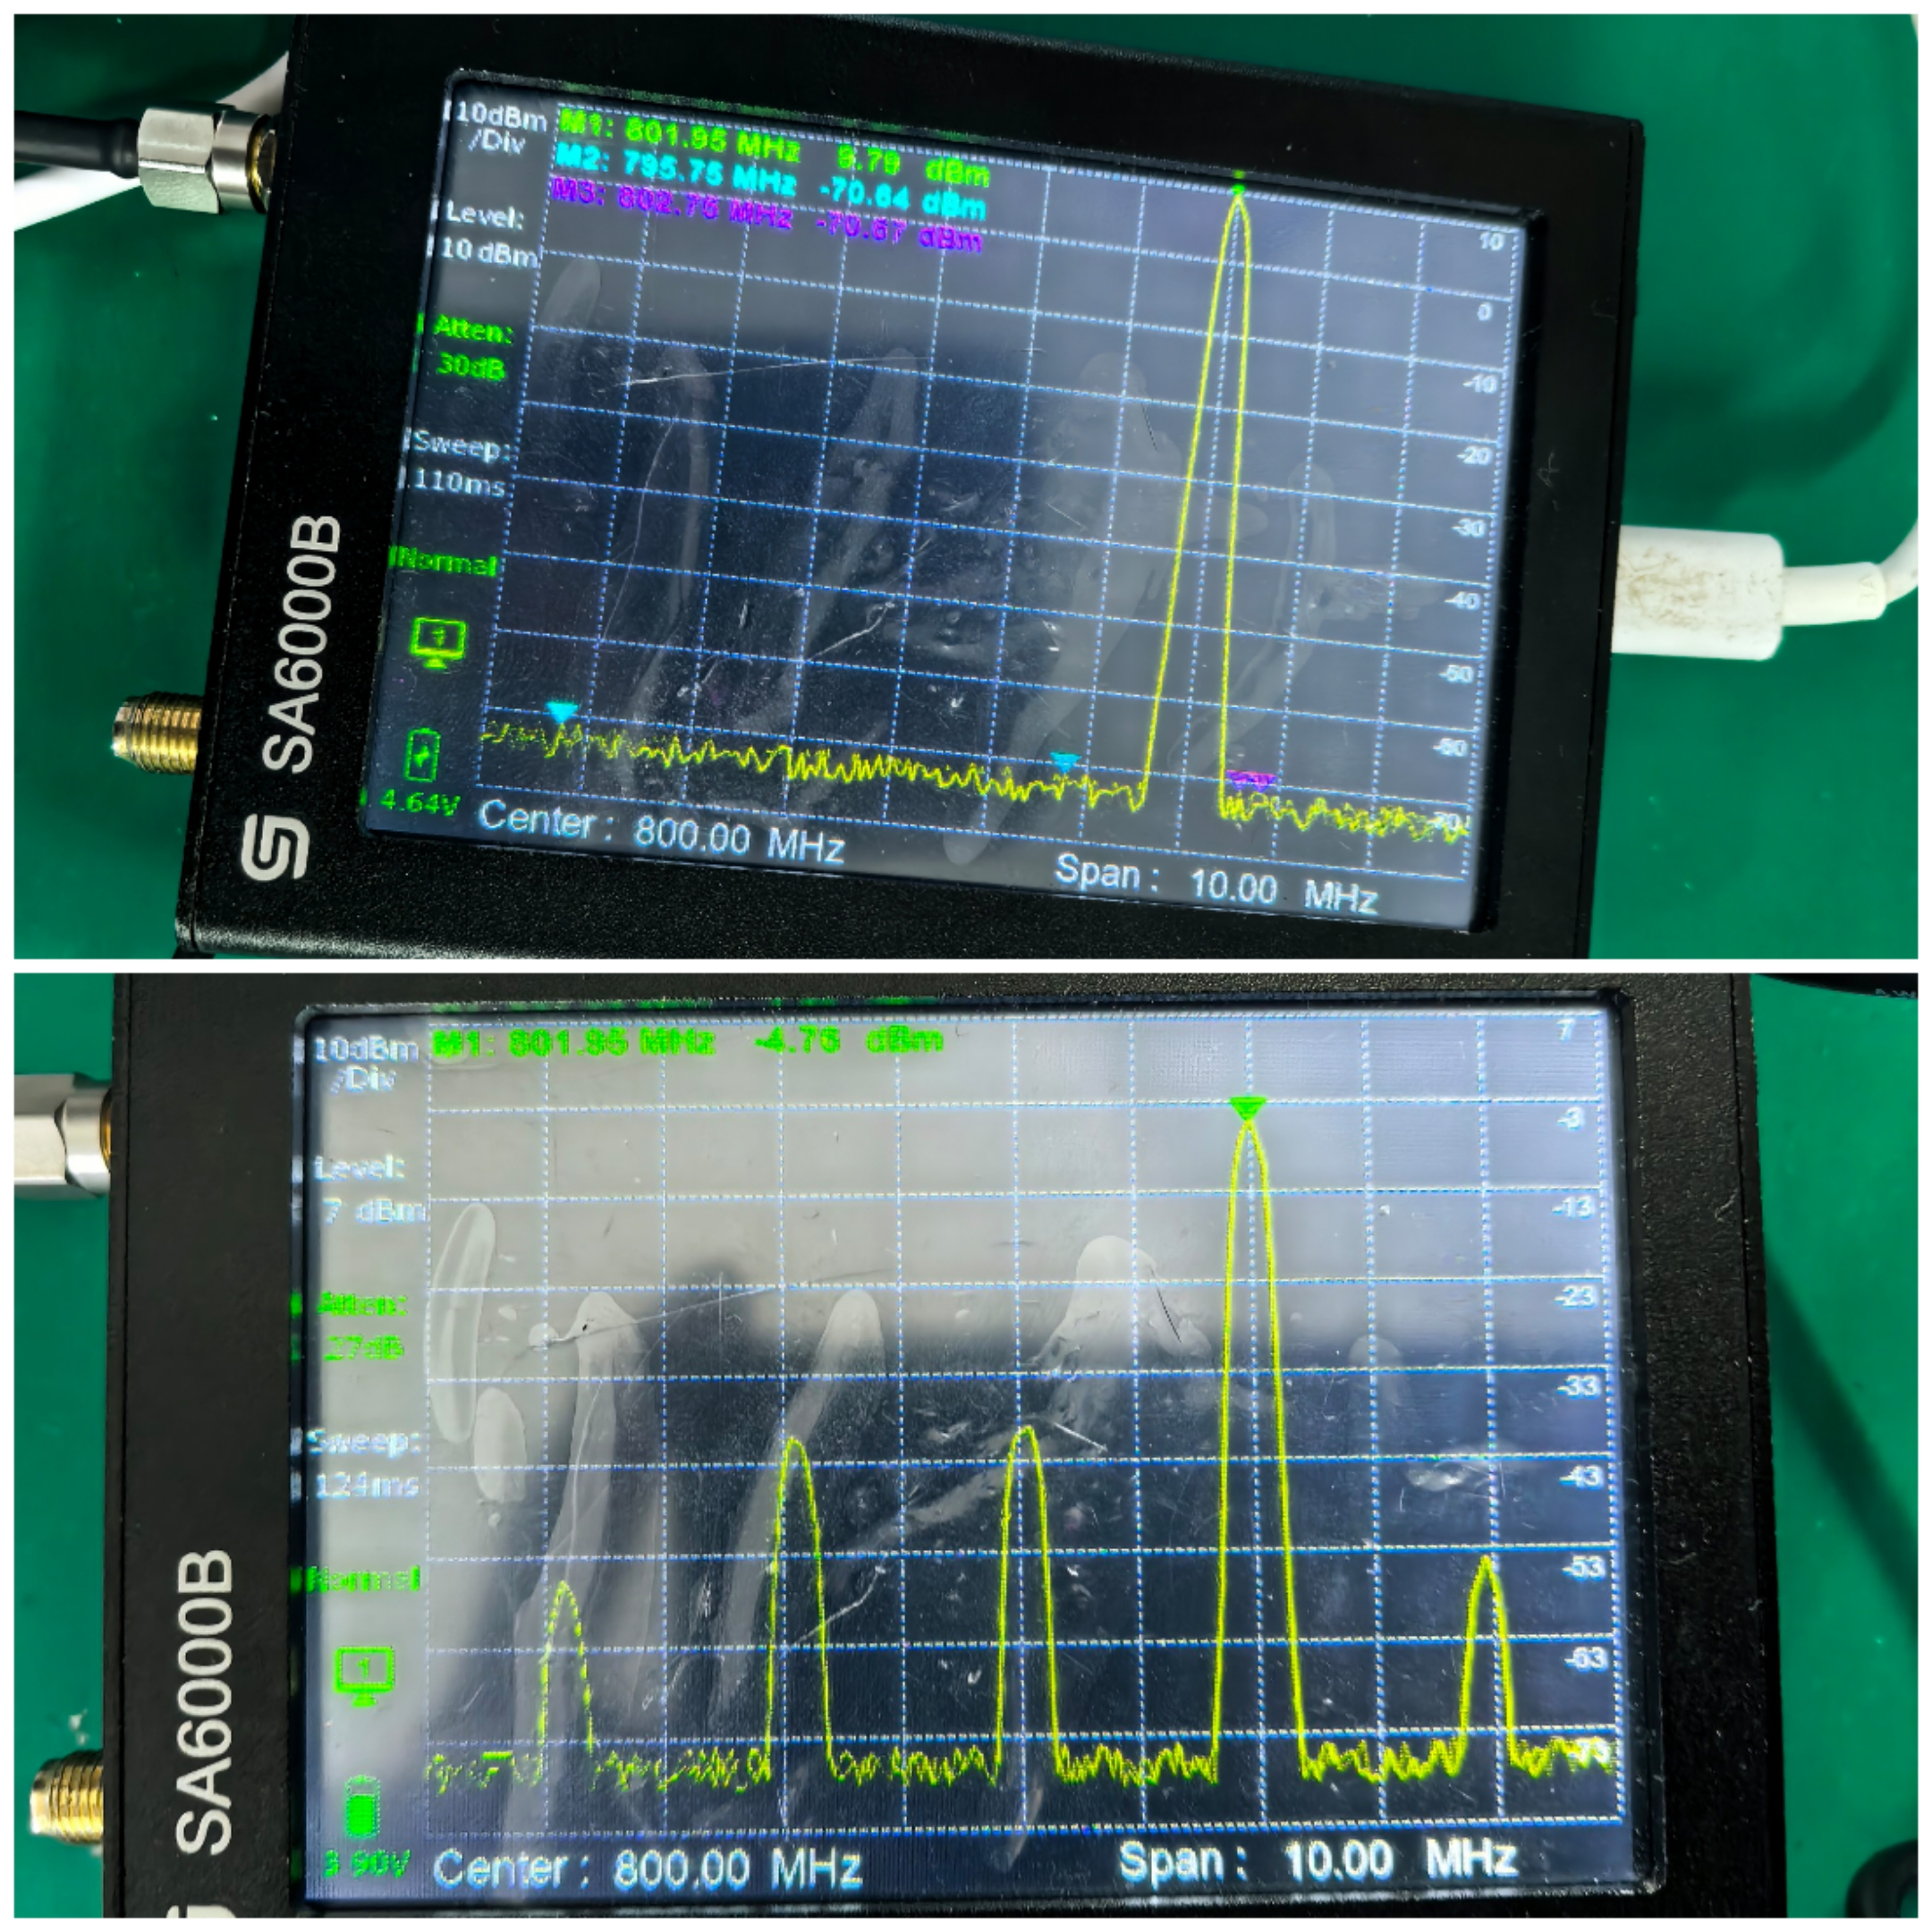
\includegraphics[width=0.8\textwidth]{picture/AD9361/AD9361 校准前后对比.jpg}
    \caption{AD9361 校准前后对比}
    \label{fig:AD9361 校准前后对比}
\end{figure}

\subsubsection{AD9361 RF and BB PLL Synthesizer配置}

AD9361 RF and BB PLL Synthesizer用于生成射频和基带信号所需的本振频率。该部分的配置首先要确定输入时钟源和输入时钟频率，FMCOMMS3评估版可以使用外部晶振作为时钟源，频率为40MHz；也可以使用外部输入时钟源，本作品选择使用40M晶振。根据寄存器手册配置TX和RX的Fref为80MHz，选择BBPLL的Fref为40MHz。

\begin{figure}[H]
    \centering
    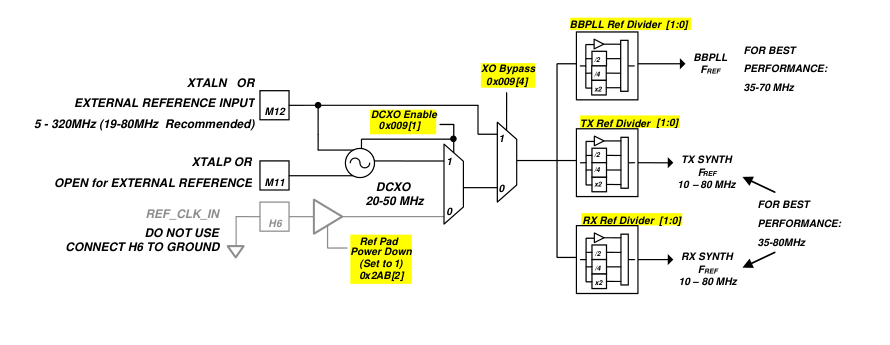
\includegraphics[width=0.8\textwidth]{picture/AD9361/AD9361输入时钟.png}
    \caption{AD9361 输入时钟}
    \label{fig:AD9361 输入时钟}
\end{figure}

根据输入的Fref和官方提供的PLL Synthesizer Block Diagram，计算出所需的PLL参数，随后进行寄存器配置即可得到所需的LO频率。

\begin{figure}[H]
    \centering
    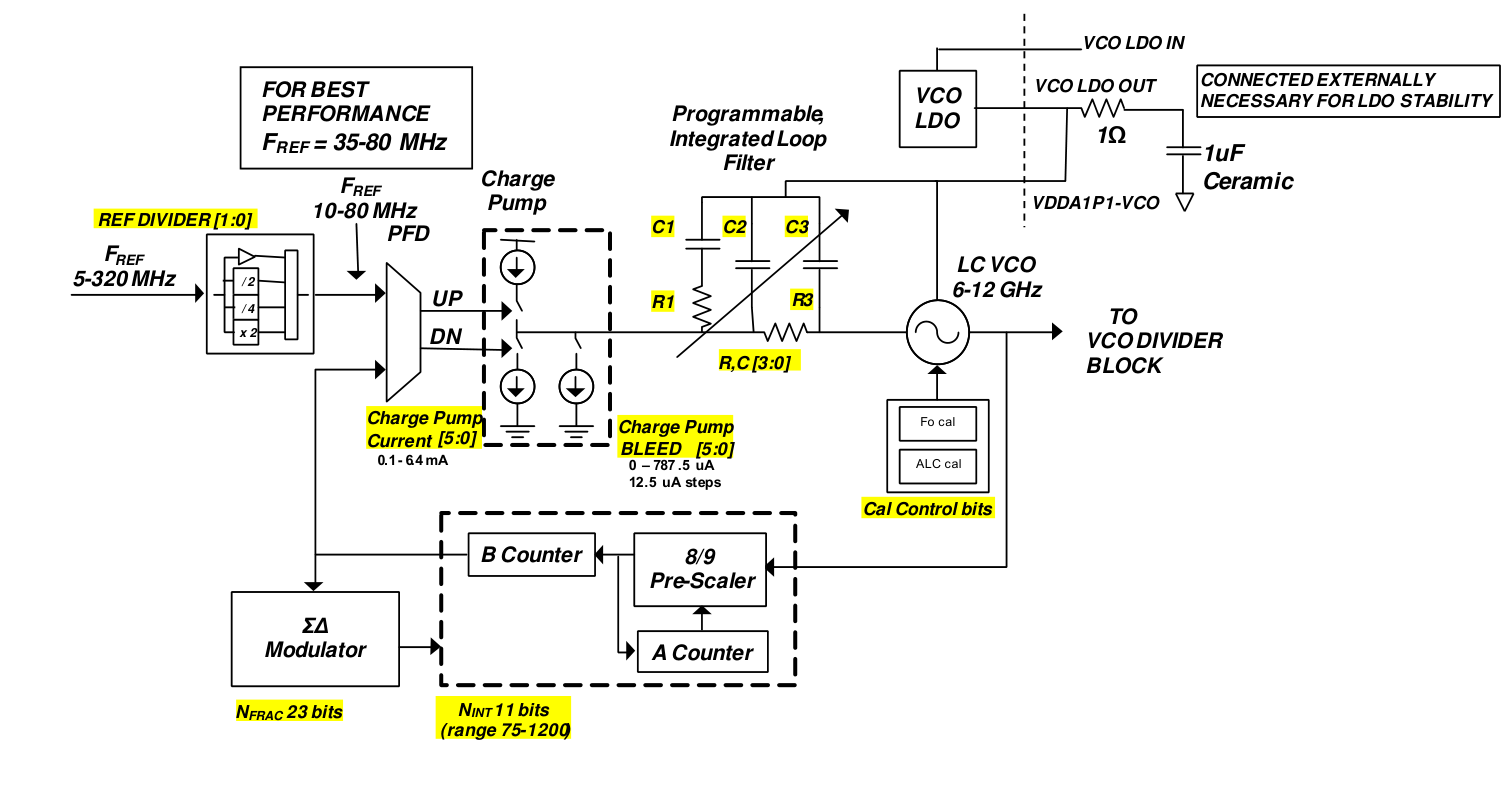
\includegraphics[width=0.8\textwidth]{picture/AD9361/AD9361 PLL.png}
    \caption{AD9361 PLL Synthesizer}
    \label{fig:AD9361 PLL Synthesizer}
\end{figure}

根据下列公式：
\begin{align*}
    F_{RFPLL} &= LO \times 2^{\text{VCO Divider} + 1} \\
    F_{RFPLL} &= F_{ref} \times \left(N_{Integer} + \frac{N_{Fractional}}{8388593}\right) \\
    N_{Fractional} &= \mathrm{Round}\left(8388593 \times \left(\frac{F_{RFPLL}}{F_{ref}} - N_{Integer}\right)\right) \\
    N_{Integer} &= \mathrm{Floor}\left(\frac{F_{RFPLL}}{F_{ref}}\right)
\end{align*}

其中，$F_{RFPLL}$为所需的RF PLL频率，$F_{ref}$为输入时钟频率，$LO$为所需的本振频率，$VCO Divider$为VCO分频器值，$N_{Integer}$为11位分频整数部分，$N_{Fractional}$为23位分频小数部分。

以及官方提供的VCO Divider选择表，可以计算出所需的PLL参数。
\begin{figure}[H]
    \centering
    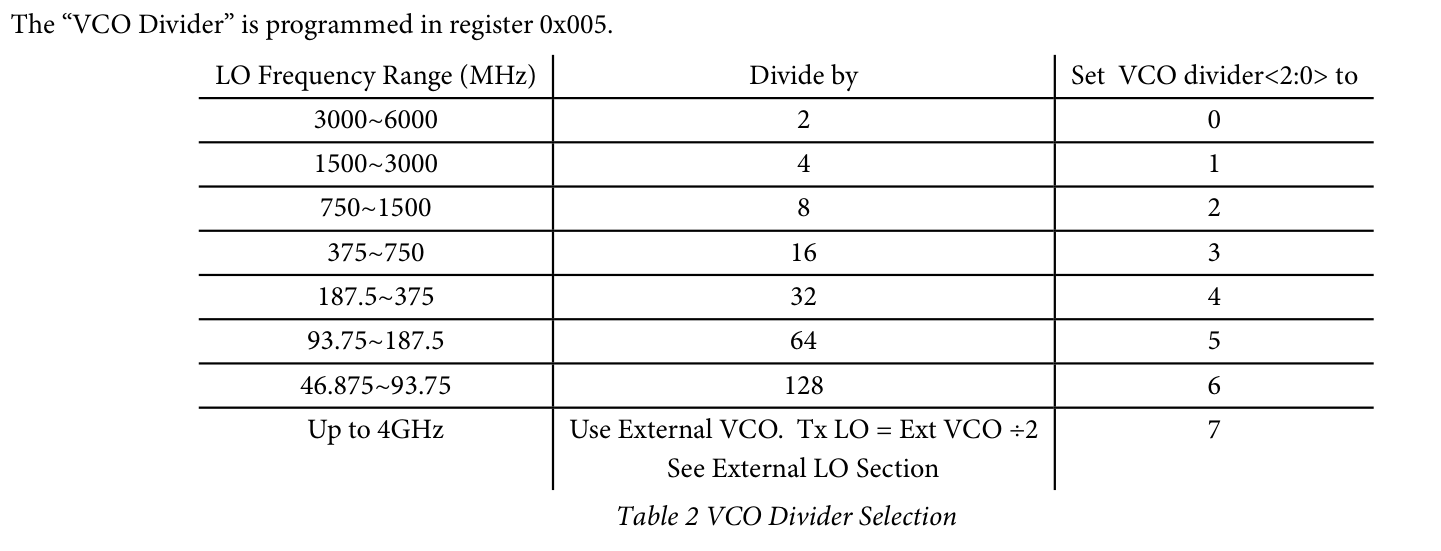
\includegraphics[width=0.8\textwidth]{picture/AD9361/VCO选择表.png}
    \caption{AD9361 VCO Divider选择表}
    \label{fig:AD9361 VCO Divider选择表}
\end{figure}

例如输出800MHz的LO频率时，选择VCO Divider为2，计算得到整数分频为80，小数分频为0。随后根据寄存器手册配置相应的寄存器值，完成PLL的配置。

BBPLL的配置会影响AD9361的采样率设置，在初始化设置时，AD9361 Evaluation Software会根据选择的采样率自动计算出BBPLL的参数，并进行相应的寄存器配置，这里不再赘述。

\subsubsection{AD9361 输出衰减配置}
AD9361支持输出衰减控制，通过控制寄存器073可以实现对输出信号的衰减。该寄存器的值范围为0-179，对应的衰减范围为0-89.5dB，步进为0.5dB。本作品根据实际需求设置合适的输出衰减值，以确保输出信号在合理范围内，避免过载或信号失真。

\subsection{电路设计}
本作品电路设计包括FPGA底板设计、功率放大器、低噪声放大器和天线的选择以及音频模块设计。
\subsubsection{FPGA底板设计}

本作品为SIPEED TANG MEGA 138K/60K核心板设计了专用的扩展底板，用于连接AD9361评估板和其他外设。底板设计主要包括电源、网口、FMC连接器和PMOD连接器等部分。

\begin{figure}[H]
    \centering
    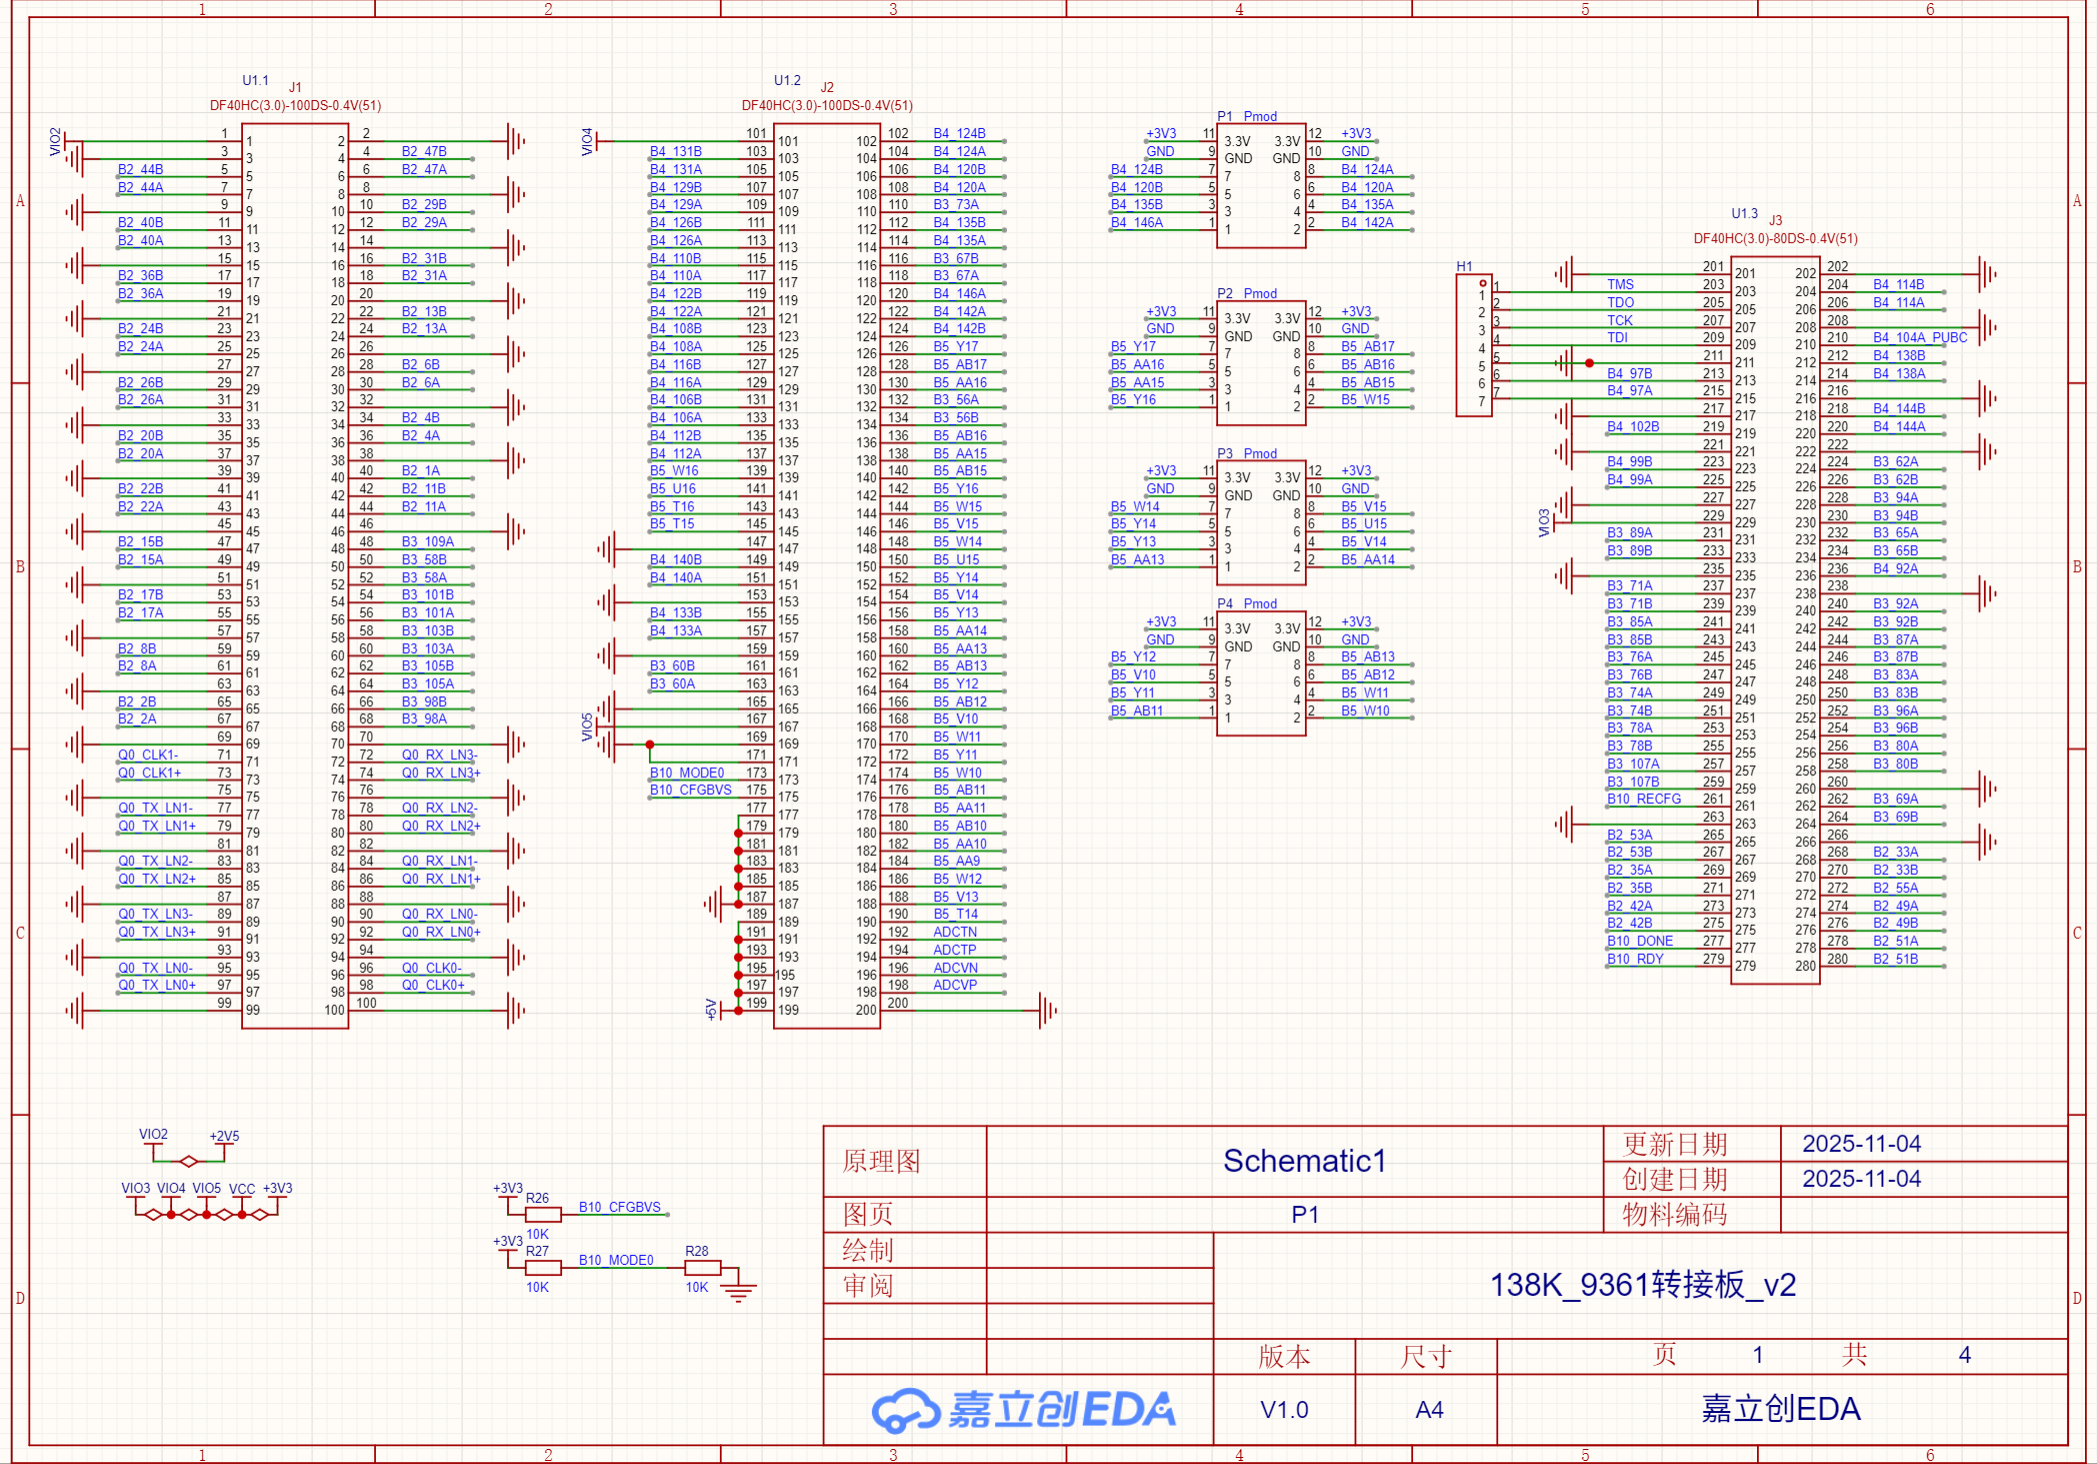
\includegraphics[width=0.8\textwidth]{picture/board/dock连接图.png}
    \caption{板对板连接器、PMOD原理图}
    \label{fig:板对板连接器原理图}
\end{figure}

该原理图主要包括板对板连接器和PMOD连接器两部分。板对板连接器用于连接TANG MEGA核心板，提供电源和信号传输通道。PMOD连接器用于连接外部模块，如传感器、显示屏等，扩展系统功能。

\begin{figure}[H]
    \centering
    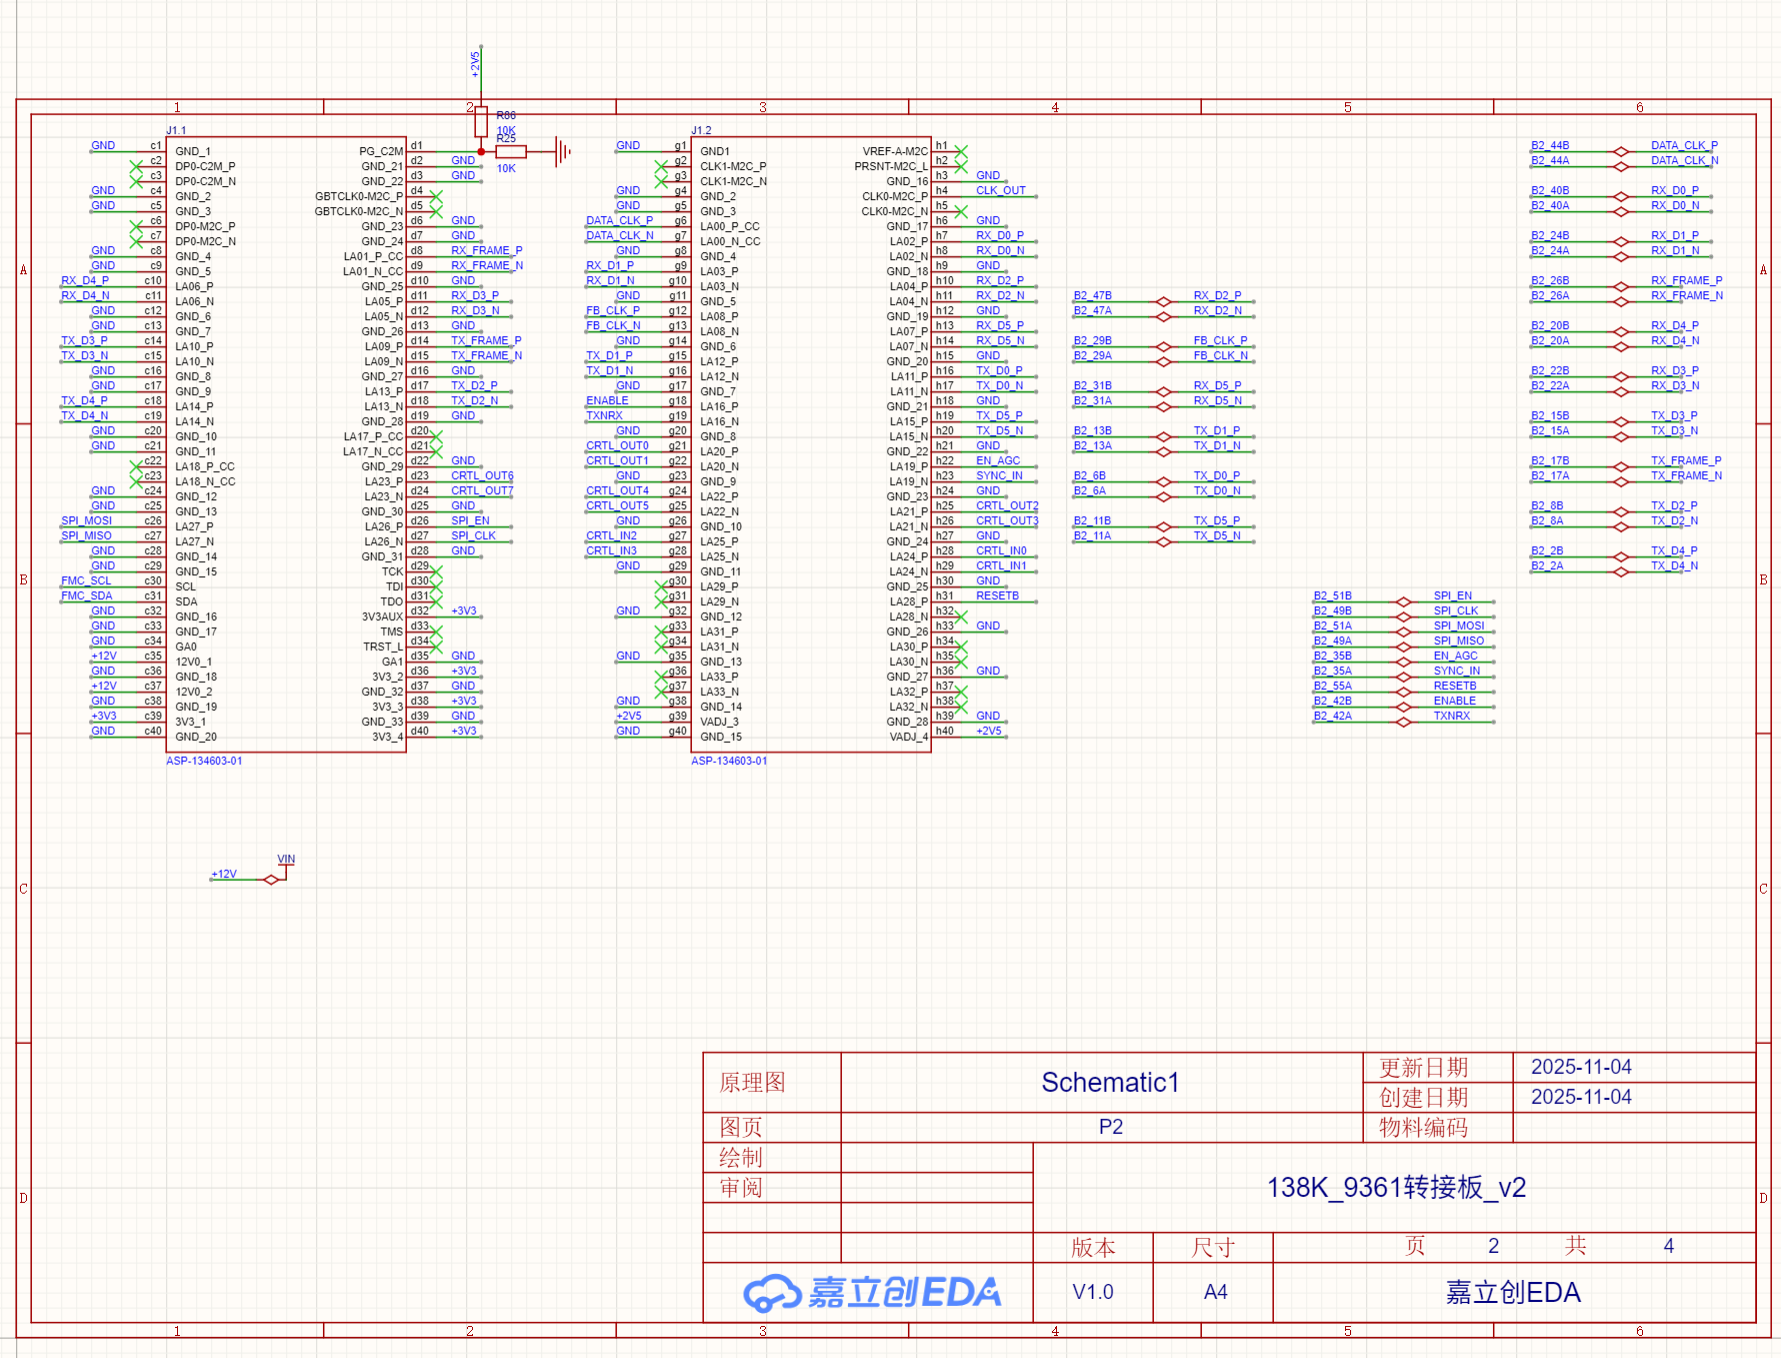
\includegraphics[width=0.8\textwidth]{picture/board/ad9361 sch.png}
    \caption{fmc电路原理图}
    \label{fig:fmc电路原理图}
\end{figure}

该原理图主要包括FMC连接器和AD9361评估板连接部分。FMC连接器用于连接AD9361评估板，提供高速数据传输通道和控制信号。设计时充分考虑了信号完整性和电磁兼容性，确保高速信号的稳定传输。

\begin{figure}[H]
    \centering
    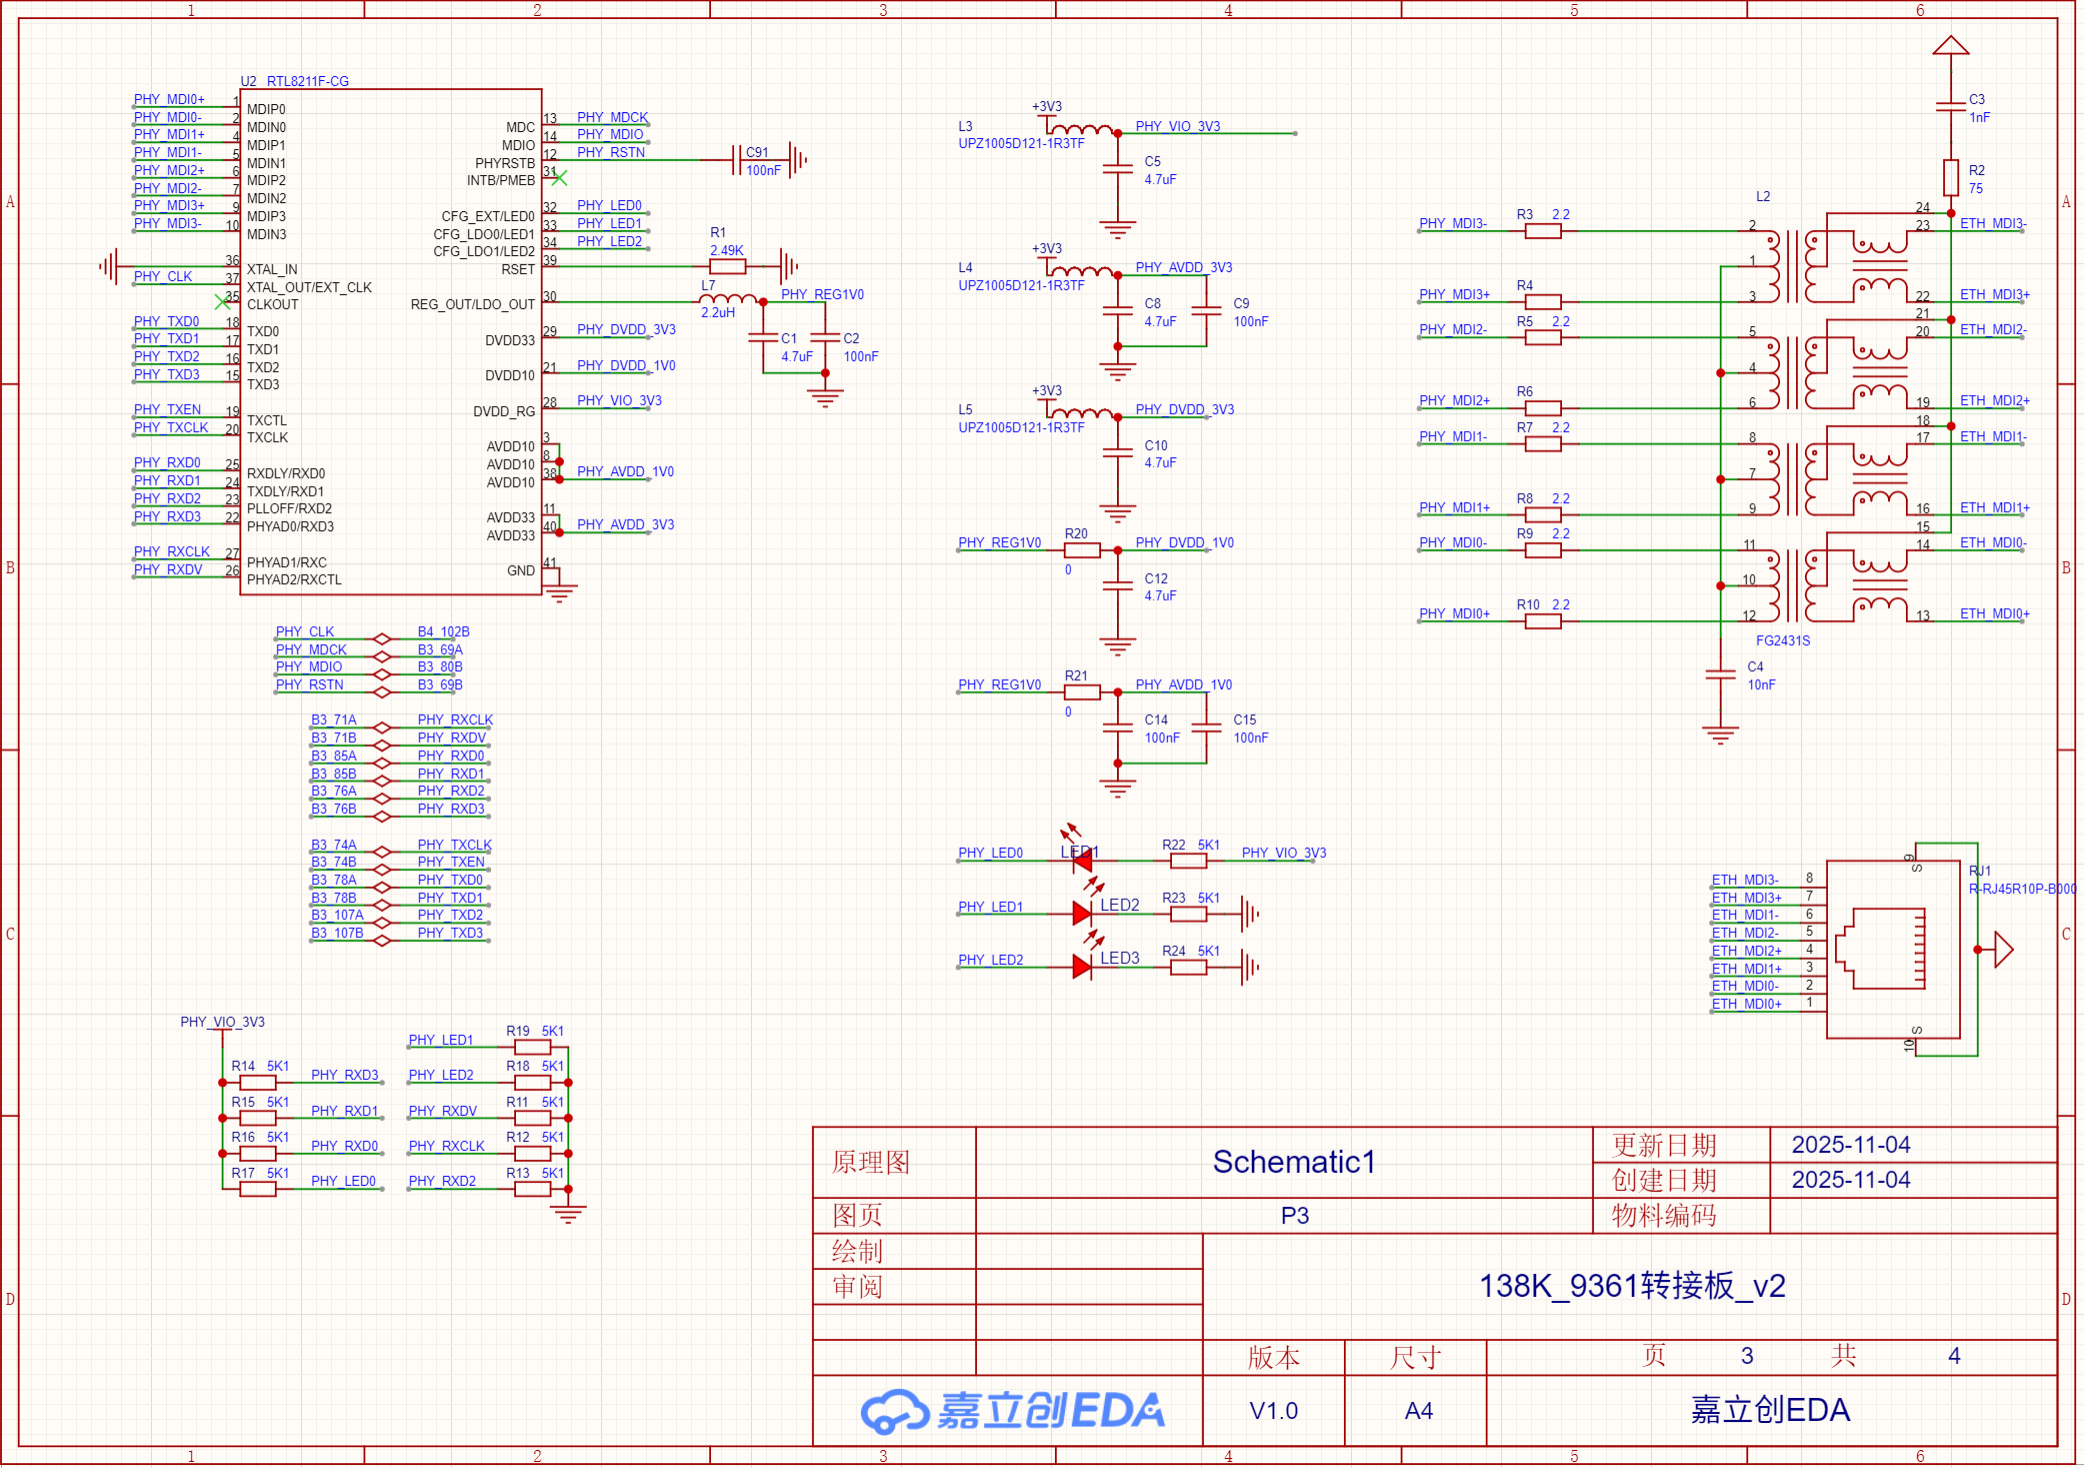
\includegraphics[width=0.8\textwidth]{picture/board/ethernet sch.png}
    \caption{网口电路原理图}
    \label{fig:网口电路原理图}
\end{figure}

该原理图主要包括以太网接口电路部分。采用常用的以太网变压器和RJ45接口，确保网络连接的稳定性和可靠性。设计时考虑了信号完整性和电磁兼容性，采用差分信号传输和适当的滤波措施，确保高速以太网信号的稳定传输。

\begin{figure}[H]
    \centering
    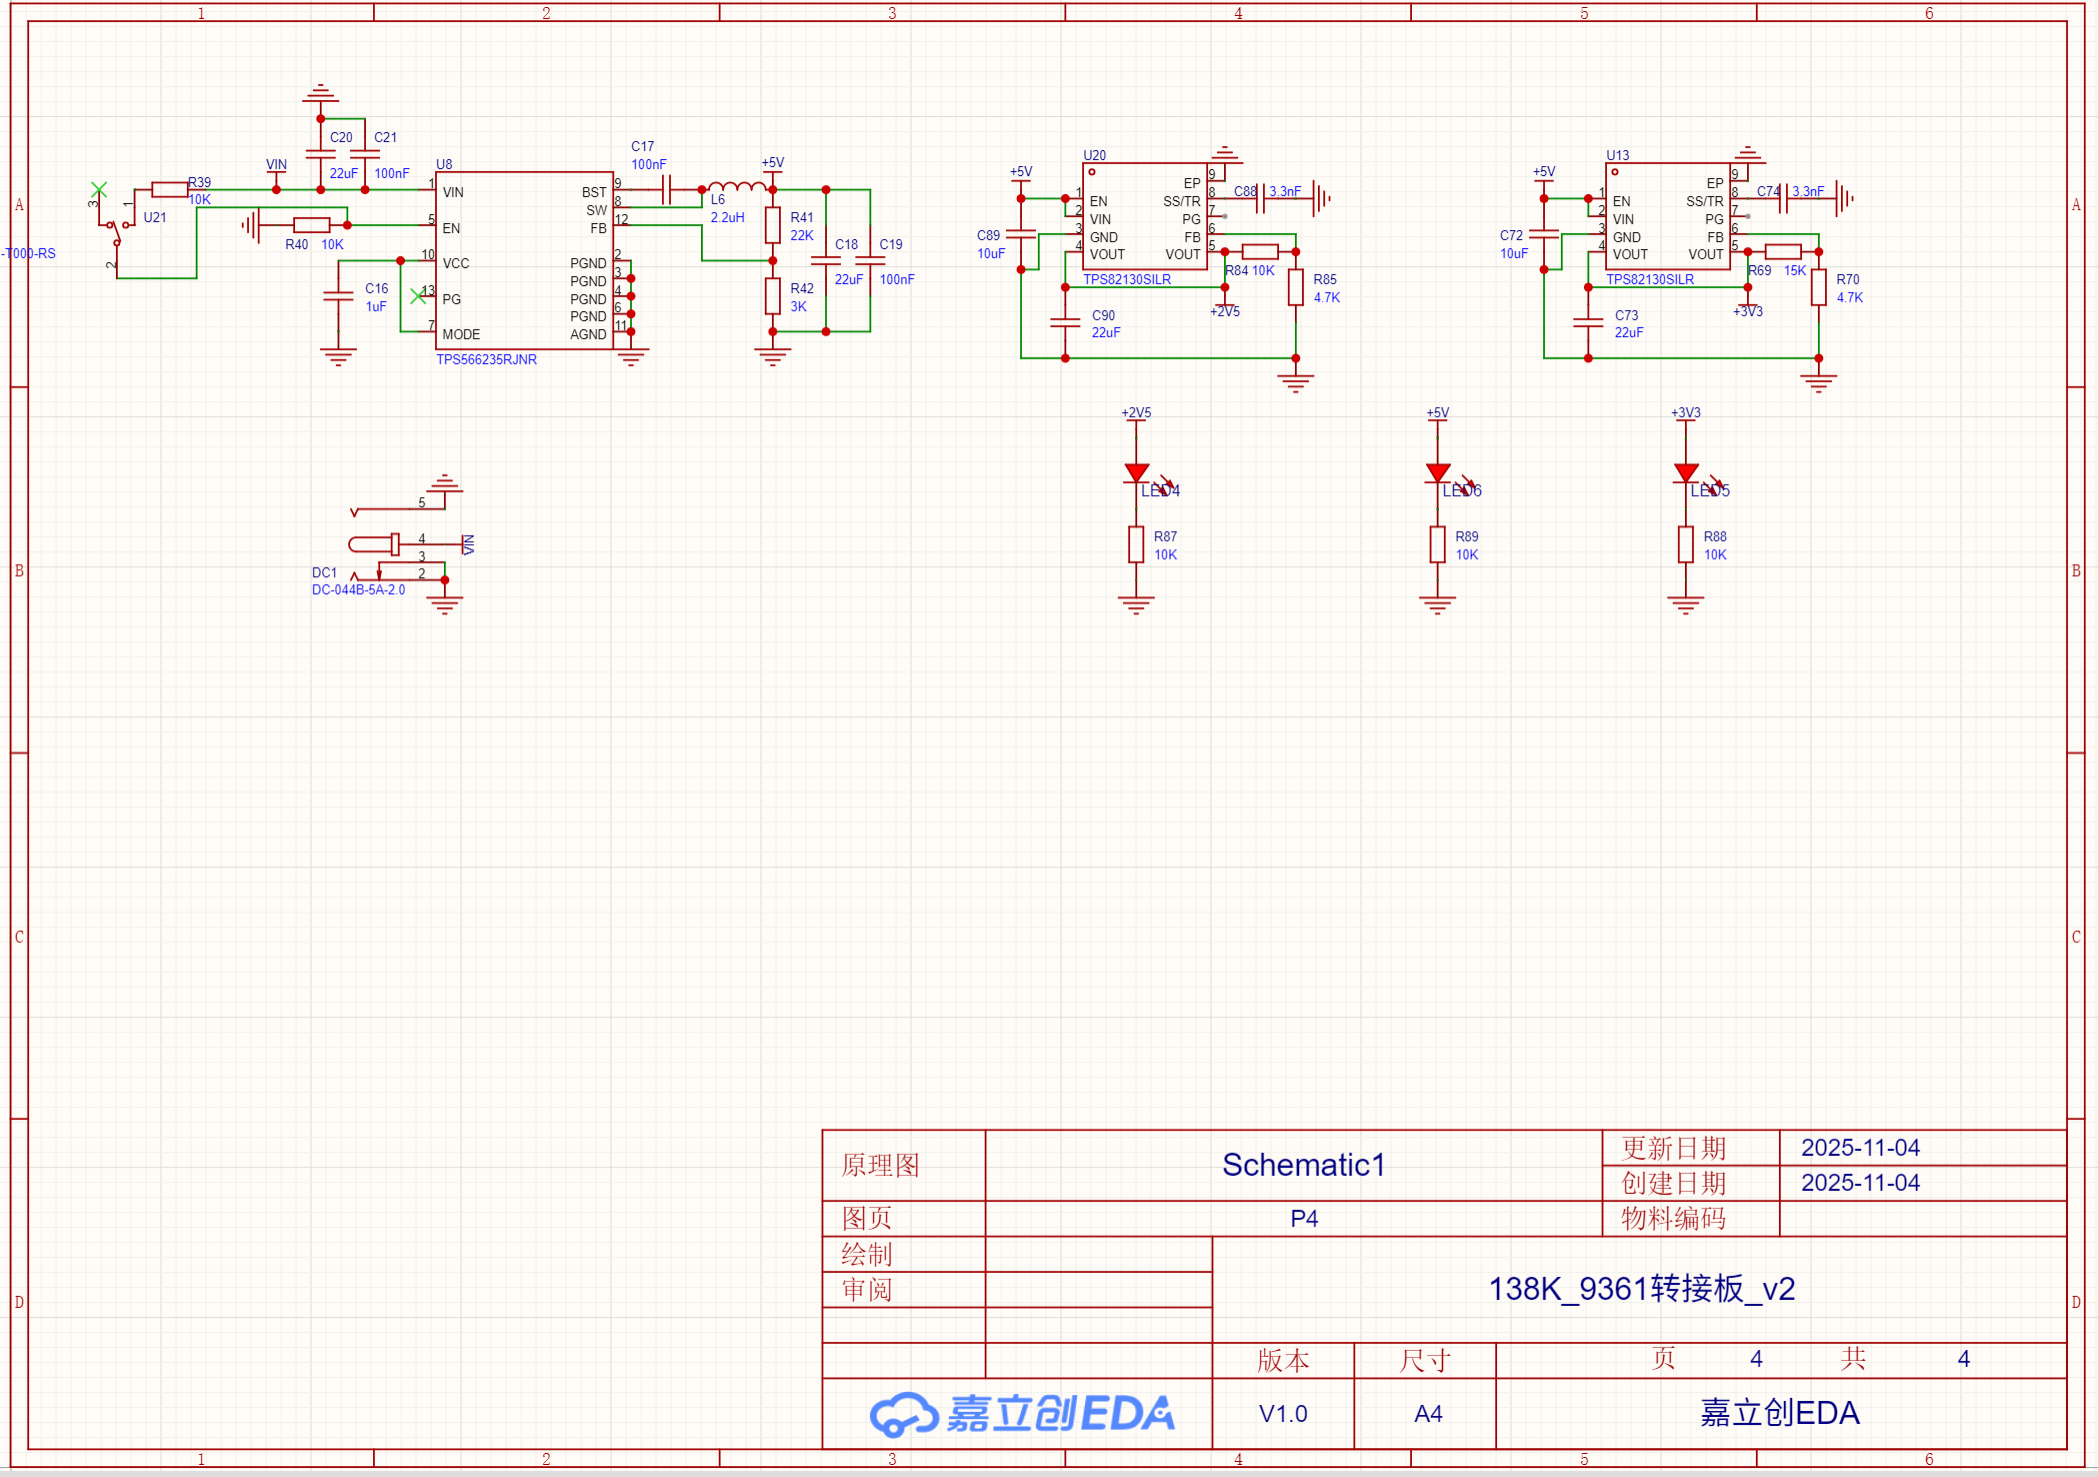
\includegraphics[width=0.8\textwidth]{picture/board/power sch.png}
    \caption{电源电路原理图}
    \label{fig:电源电路原理图}
\end{figure}

该原理图主要包括电源管理部分。采用多路稳压芯片，为各个模块提供稳定的电源供应。设计时充分考虑了电源噪声和干扰，采用滤波和去耦措施，确保系统的稳定运行。

\begin{figure}[H]
    \centering
    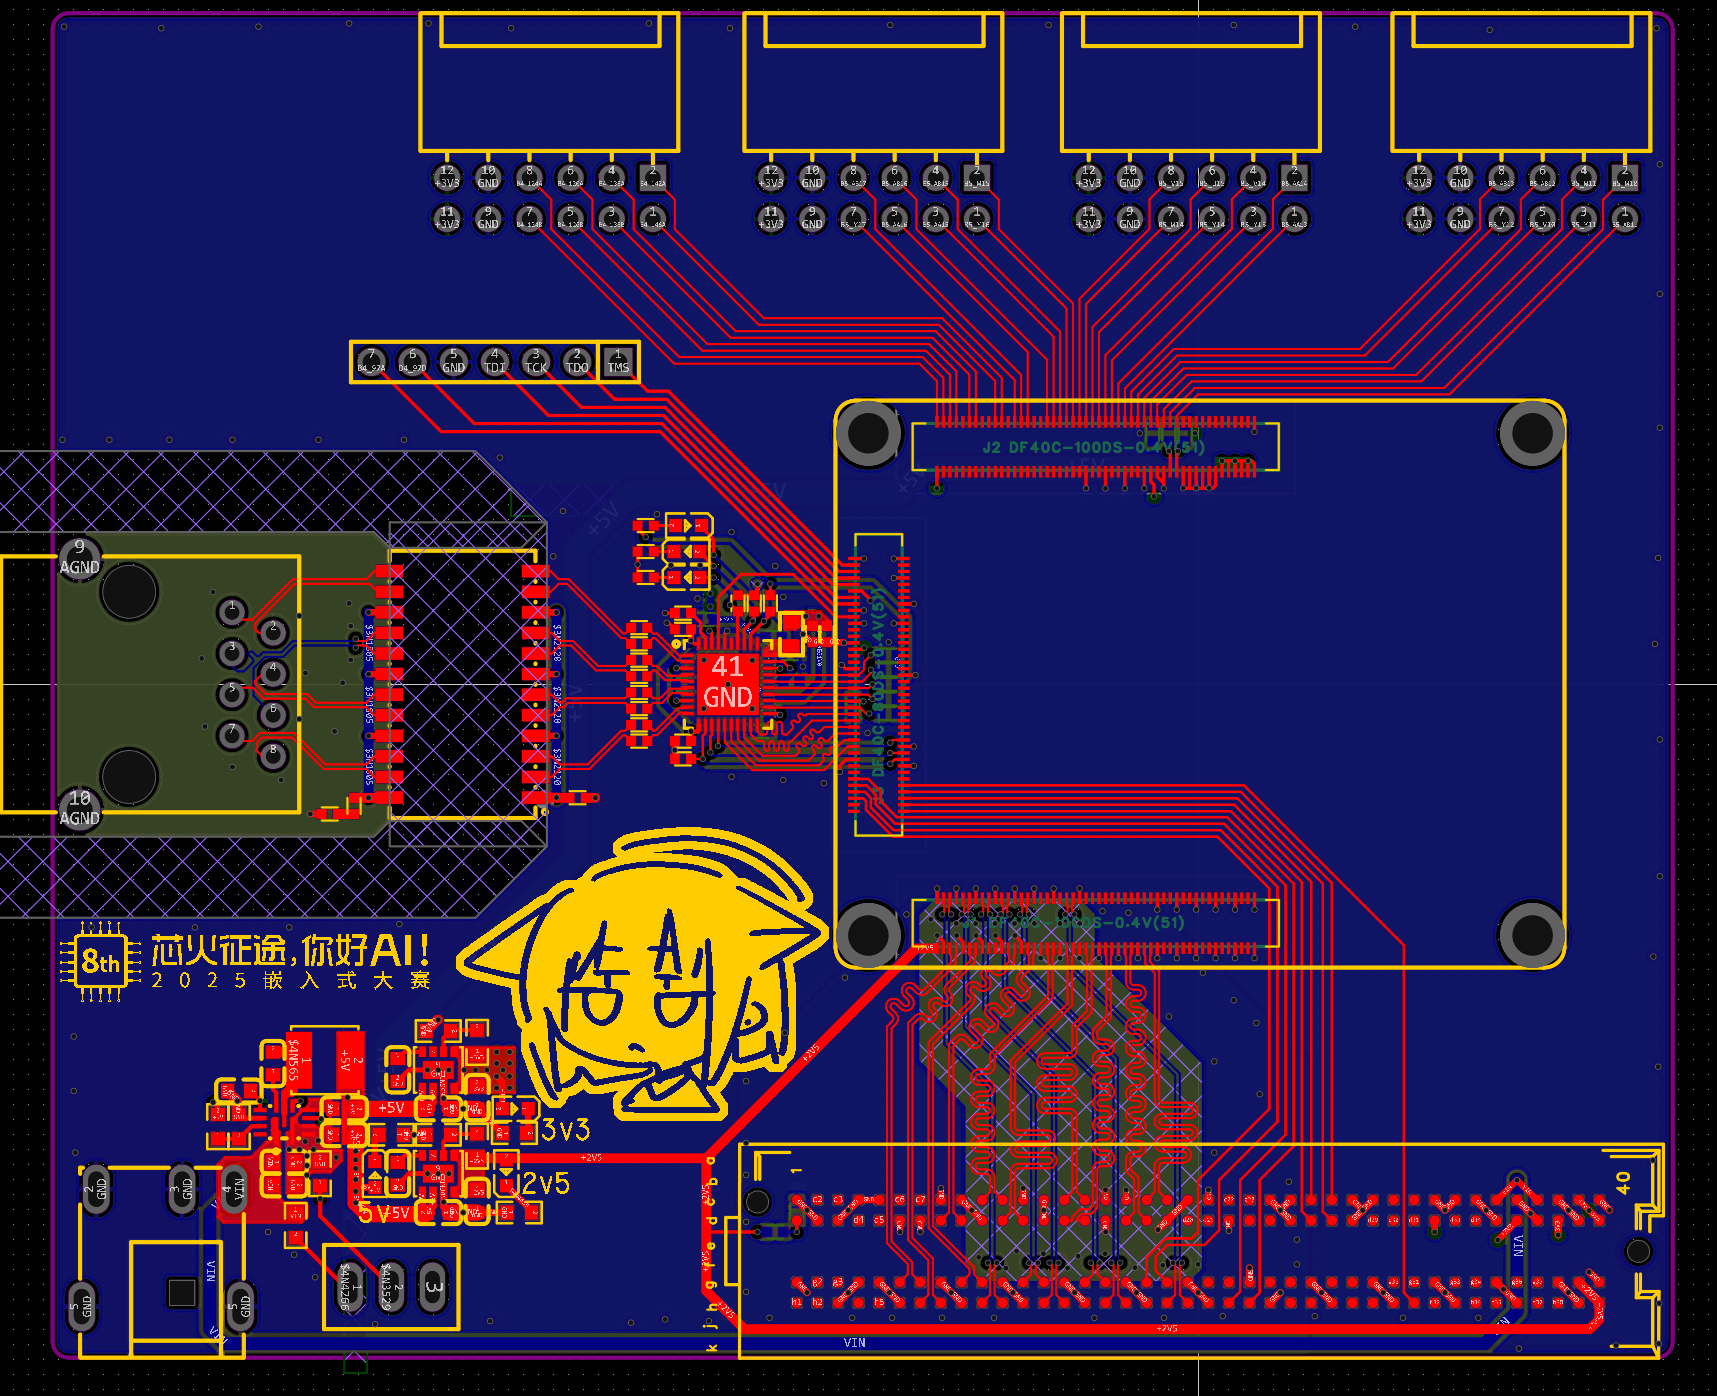
\includegraphics[width=0.8\textwidth]{picture/board/pcb.png}
    \caption{底板PCB设计}
    \label{fig:底板PCB设计}
\end{figure}

在设计底板PCB时，充分考虑了信号完整性和电磁兼容性，采用多层板设计，合理布线和接地，确保系统的稳定运行。在FMC高速接口、网口接口部分设计充分考虑了走线的等长，底板设计完成后，进行了严格的测试和验证，确保各个模块功能正常，满足设计要求。

\subsubsection{功率放大器、低噪声放大器、天线}

\subsubsection{音频模块}
本作品的音频模块选择了MAX98357A芯片，该芯片使用标准IIS协议，支持最高96KHz采样率，32位数据精度。

\begin{figure}[H]
    \centering
    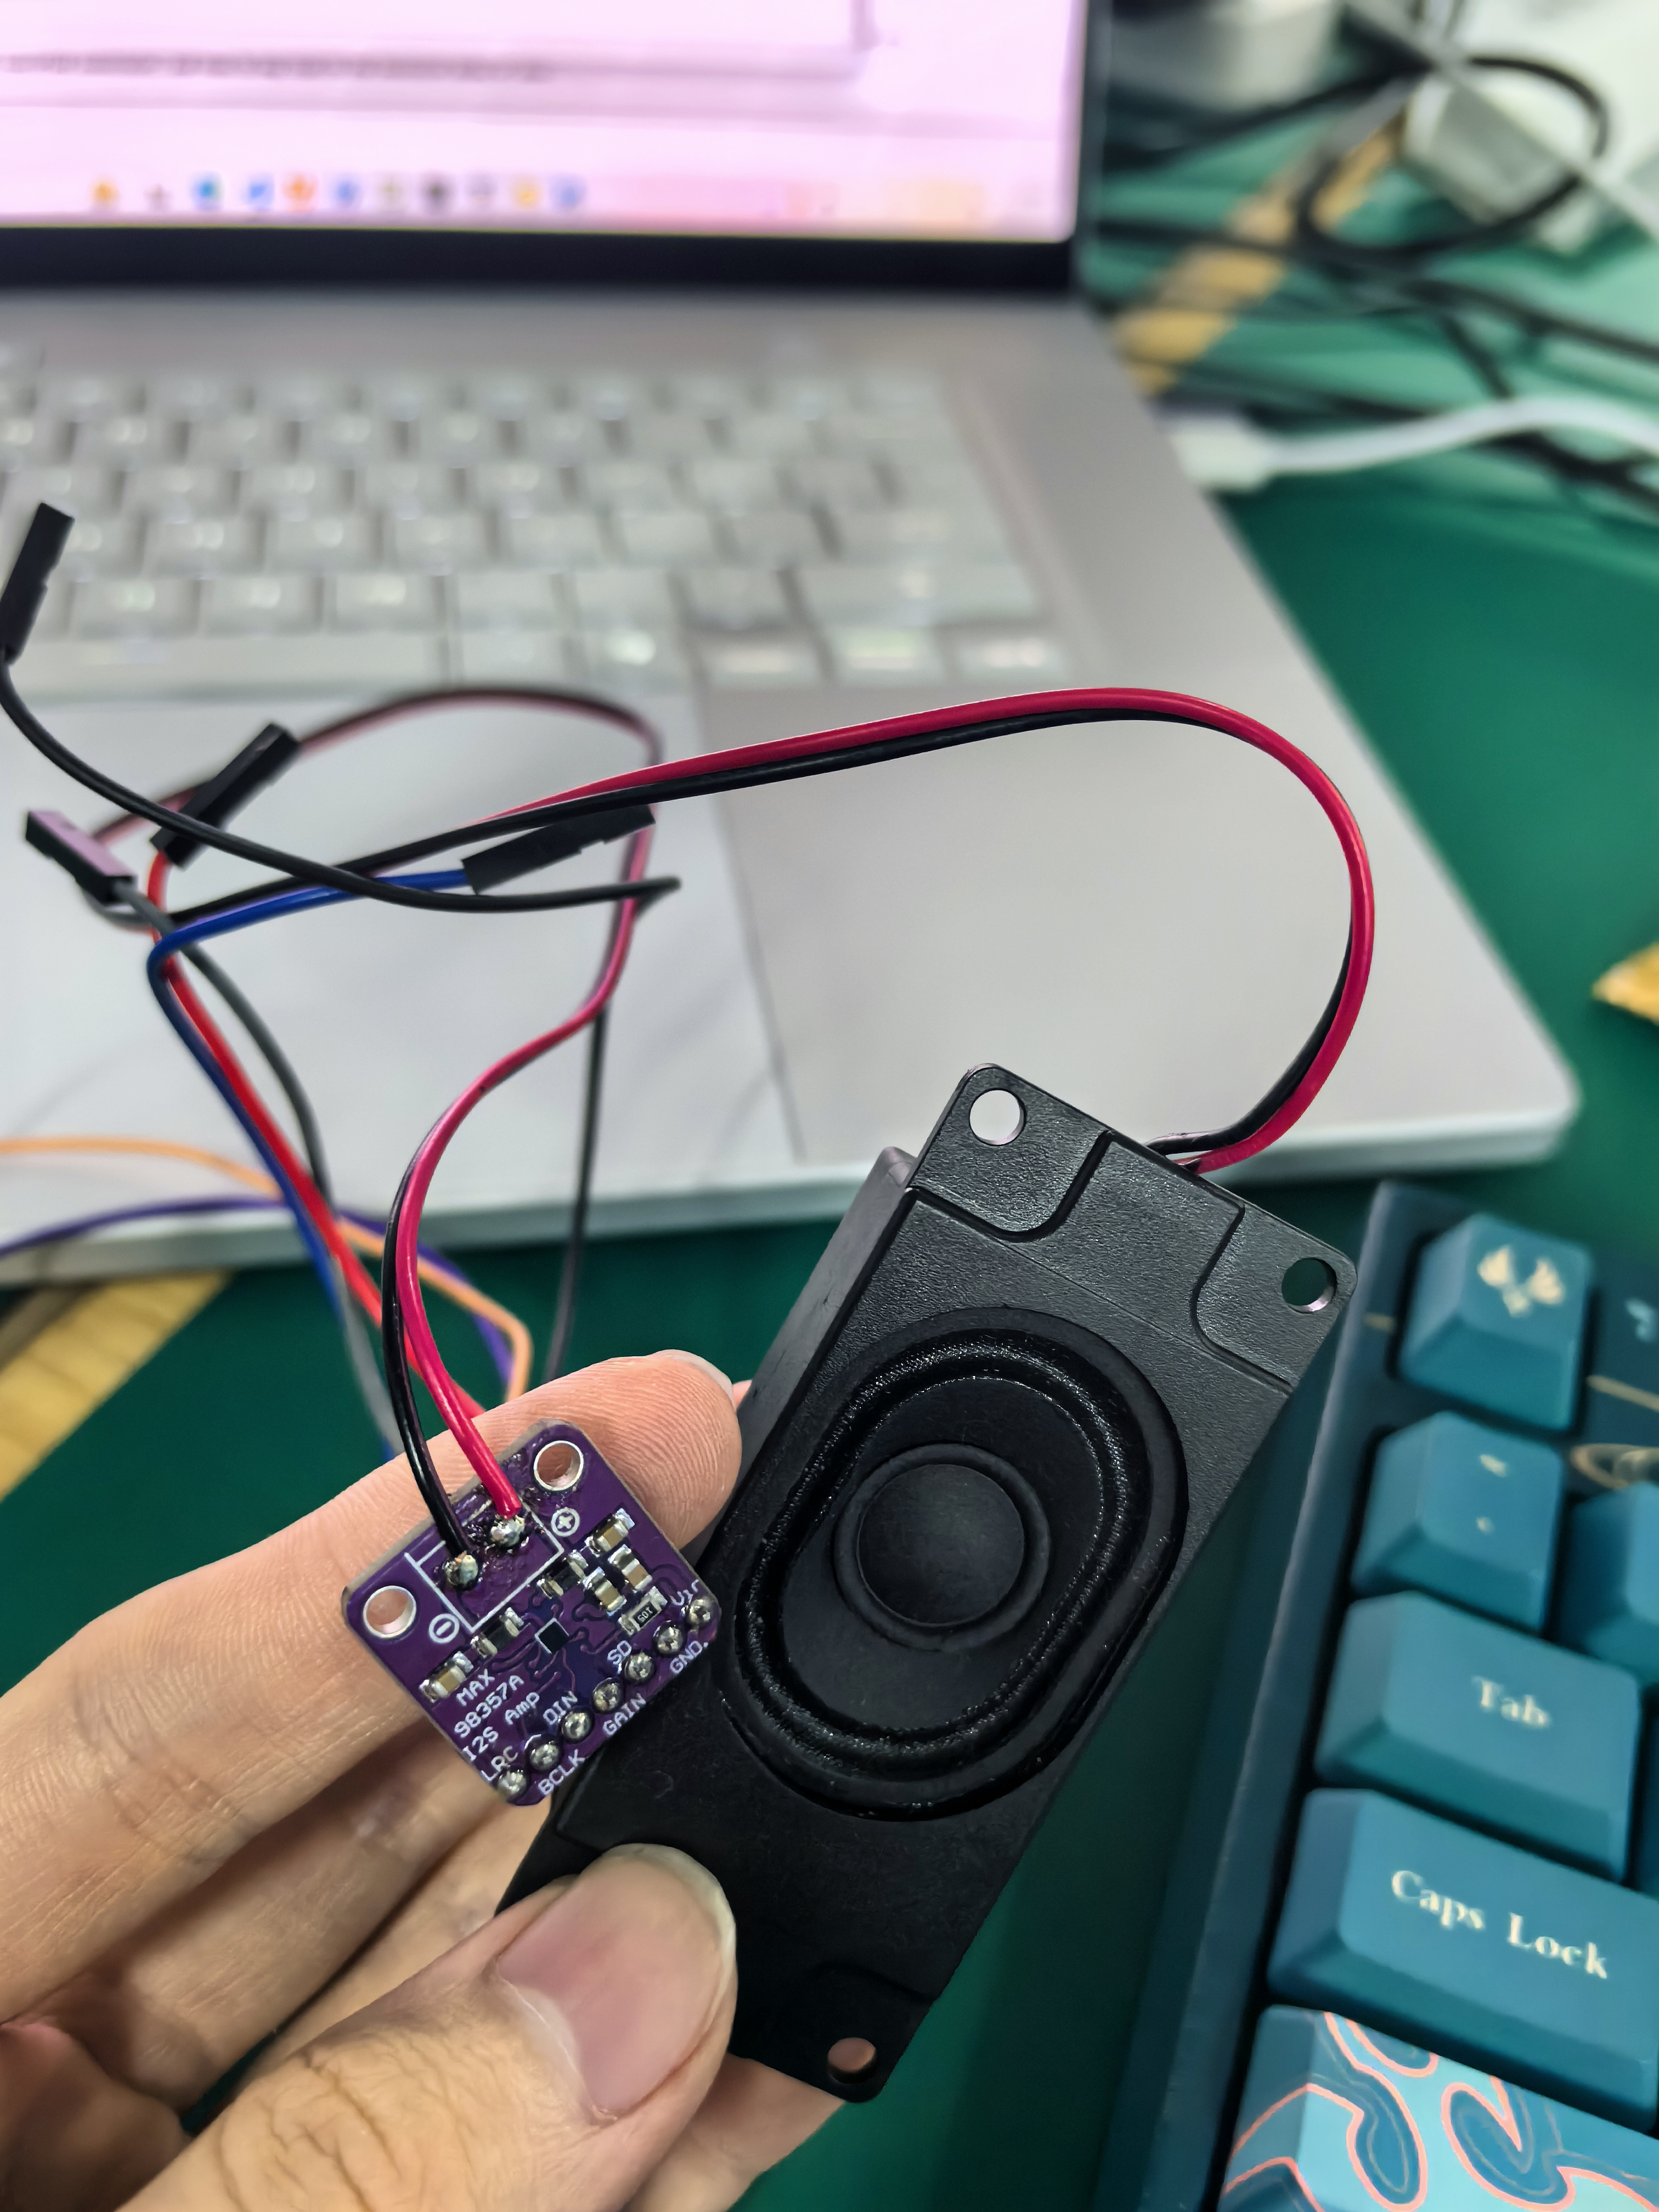
\includegraphics[width=0.8\textwidth]{picture/board/MAX 98357A.jpg}
    \caption{音频模块}
    \label{fig:音频模块}
\end{figure}

% 第三部分：完成情况及性能参数
\section{完成情况及性能参数}

\subsection{作品照片}
整个系统实物的正面、斜45°全局性照片。

\subsection{工程成果}
\subsubsection{电路成果}
电路成果实物照片。

\subsubsection{软件成果}
软件界面照片。

\subsection{特性成果}
逐个展示功能、性能参数等量化指标。可加重要仪器测试或现场照片。

% 第四部分：总结
\section{总结}

\subsection{可扩展之处}
本作品实现了简单的无线通信系统，能够在两个设备之间进行数据传输，能够解调FM广播信号并播放音频。系统设计具有一定的灵活性和可扩展性，未来可以在以下几个方面进行改进和扩展：
\begin{itemize}[leftmargin=*]
    \item 增加更多的调制方式：目前系统仅支持8PSK调制，未来可以增加更多的调制方式，如QPSK、16QAM等，以适应不同的应用需求。
    \item 提高数据传输速率：通过优化信道编码和调制方案，可以进一步提高数据传输速率，满足更高带宽需求的应用场景。
    \item 增强抗干扰能力：引入更先进的信道编码技术和频率跳变技术，提高系统在复杂无线环境下的抗干扰能力。
    \item 支持多用户通信：实现多用户接入和资源分配机制，支持多个设备同时进行通信，提高系统的利用率。
    \item 更高的实用性：增加与实际应用相关的功能模块，如蓝牙模块、Wi-Fi模块等，提升系统的实用性和应用范围。
    \item 集成更多功能模块：如GPS定位模块、传感器接口等，扩展系统的应用范围。
    \item 优化功耗管理：通过硬件和软件优化，降低系统功耗，延长设备的使用时间。
\end{itemize}

\subsection{心得体会}
在本次作品的设计与实现过程中，我完整经历了从需求分析、硬件选型、FPGA 开发到上位机软件调试的全过程。硬件方面选择 AD9361 评估板作为射频前端，结合 GOWIN FPGA 实现数据接口与时序控制，过程中对 LVDS 时序、IODELAY 调整、IQ 校准和 DC 偏移校正等环节做了大量上板验证，确保射频链路与数字接口在实际板级环境中可靠工作。软件方面，基于 Python/Qt 实现了上位机，负责寄存器配置、时延/增益调参与数据显示，提升了系统的可控性和可重复验证性。

在发送端，我们把以太网收到的字节流放入输入 FIFO，通过位宽转换将 8bit 字节映射为适用于 8PSK 的符号序列，然后进行差分编码并通过查表输出定点格式的 I/Q 样点。为满足 AD9361 对采样率和带外抑制的要求，设计了插值与成形滤波器（可采用多级 CIC 与 FIR 或升余弦成形），并在仿真中确定了滤波系数与内部位宽以避免溢出。最终的数字样点被拆分并按 LVDS DDR 时序打包输出，使用 IODELAY 进行精细时序调整，保证在物理链路上的稳定传输。

接收端实现了完整的 LVDS 重组与前端处理流程：从差分输入到单端化、通过 IODELAY 与寄存器协同定位并拼接成 12 位采样，随后进行抽取与匹配滤波以提升信噪比。载波与符号时钟恢复采用 Costas 环路与，这些环路参数可在上位机上调节以适应不同的频偏和 SNR 条件。经由判决器将相位映射回数字符号后，使用差分解码与帧头/CRC 校验恢复出稳定的字节流并通过 FIFO 传回上位机进行后续处理。

在实现层面我们采用了定点算术（内部 I/Q 通常采用 16–24 位）来在保证精度的同时节省资源，并通过 ROM 查表、多相/FIR 优化和流水线化来降低 DSP 和 BRAM 的占用、提升时钟频率。验证环节以仿真、vcd 波形调试和环回测试为主：先在仿真环境用 icarus 等工具验证模块功能，再通过 FPGA→AD9361→FPGA 的环回验证端到端链路、记录关键寄存器与测试截图以保证结果可复现。

在射频部分遇到的主要挑战包括：LVDS 接口的时序对齐（需协调 AD9361 寄存器与 FPGA IODELAY）、校准流程的自动化以及在噪声与镜像干扰条件下的 IQ 校正。为解决这些问题，我先在仿真与板级自检模式下定位时序偏移，然后结合寄存器配置与 FPGA 内部延时原语细调，最终通过频谱与示波器验证了校准效果。此外，文档化每一步配置流程与寄存器表，有助于后续复现和参数迁移。

总体而言，这次工程不仅巩固了我们在数字基带算法（包括 8PSK 的映射与判决、插值/抽取滤波、环路与时序恢复）方面的实现能力，也增强了我在 FPGA 与射频前端协同调试、测试流程建设以及参数化设计方面的经验。下一步工作将聚焦于把校准流程进一步脚本化（例如自动化 IODELAY 扫描和 IQ/mirror 校准）、增加更多可配置的调制格式与滤波参数，并把测试向量与结果套件化以便快速回归验证。

通过本次开发，我们在射频与数字接口协同调试、PLL/滤波器参数理解、以及系统化测试流程建设方面都有较大收获。后续可改进之处包括：把校准流程进一步自动化（脚本化 IQ/镜像/LO 校准），把图片和寄存器输出结果集成为可回放的测试套件，以及将图像文件名规范化以避免跨平台路径问题。总的来说，本次项目锻炼了我从系统设计到上板验证的完整能力，也为后续功能扩展（更多调制方式、更高带宽）打下了扎实基础。

% 第五部分：参考文献
% \section{参考文献}
% \begin{enumerate}[leftmargin=*]
%     \item 参考文献1
%     \item 参考文献2
%     \item ……
% \end{enumerate}

\end{document}